% Use only LaTeX2e, calling the article.cls class and 12-point type.

\documentclass[11pt]{article}
\usepackage[round,semicolon]{natbib}
\usepackage[margin=1.4in]{geometry}
\usepackage{kpfonts}

\usepackage{seqsplit}
\usepackage{placeins}

\usepackage{newfloat}
\usepackage[labelfont=bf]{caption}
\usepackage{nameref}
\usepackage{rotating}
\usepackage{color}
\usepackage{float}

\setcounter{topnumber}{8}
\setcounter{bottomnumber}{8}
\setcounter{totalnumber}{8}
\renewcommand{\topfraction}{1}
\renewcommand{\bottomfraction}{1}
\renewcommand{\textfraction}{0}
\renewcommand{\floatpagefraction}{1}

\usepackage[font=small,labelfont=bf]{caption}

\usepackage{newfloat}
\DeclareFloatingEnvironment[name={Figure}]{suppfigure}
\renewcommand{\thesuppfigure}{S\arabic{suppfigure}}

\definecolor{darkblue}{rgb}{0, 0.0, 0.6}

\usepackage{hyperref}
\hypersetup{colorlinks,citecolor=blue,linkcolor=blue,urlcolor=blue}

\usepackage{seqsplit}

\usepackage{array}
\newcolumntype{R}[1]{>{\raggedright\arraybackslash}p{#1}}
\newcolumntype{C}[1]{>{\centering\let\newline\\\arraybackslash\hspace{0pt}}m{#1}}

\newcommand{\comment}[1]{{\color{red}[\textsl{#1}]}}

\usepackage{setspace}

\renewcommand{\topfraction}{1}
\renewcommand{\bottomfraction}{1}
\renewcommand{\textfraction}{0}
\renewcommand{\floatpagefraction}{1}

%\renewcommand{\abstractname}{\large SUMMARY}


\title{Quantifying the ease of viral escape from broad and narrow antibodies to influenza hemagglutinin} 

\author
{Michael B. Doud$^{1,2,3,\dagger}$, Juhye M. Lee$^{1,2,3,\dagger}$, and Jesse D. Bloom$^{1,2,*}$\\
\\
\scriptsize{$^1$Basic Sciences and Computational Biology Program, Fred Hutchinson Cancer Research Center}\\
\scriptsize{$^2$Department of Genome Sciences and $^3$Medical Scientist Training Program, University of Washington} \\
\scriptsize{Seattle, WA, USA} \\
\scriptsize{$^{\dagger}$These authors contributed equally} \\
\scriptsize{$^*$Correspondence: \href{jbloom@fredhutch.org}{jbloom@fredhutch.org}}
}

\date{}


\begin{document}

\maketitle
\onehalfspacing

\begin{abstract}
Influenza virus can completely escape most antibodies with single mutations.
However, rare antibodies broadly neutralize many viral strains.
It is unclear how easily influenza virus might escape such antibodies if they became widespread due to therapeutic use or vaccination.
Here we map all single amino-acid mutations that increase resistance to broad antibodies targeting an H1 hemagglutinin.
Crucially, our approach not only identifies antigenic mutations but also quantifies their effect sizes.
All antibodies select mutations, but the effect sizes vary widely. 
The virus can escape a broad antibody targeting hemagglutinin's receptor-binding site the same way it escapes narrow strain-specific antibodies: via single mutations with huge effects.   
In contrast, broad antibodies targeting hemagglutinin's stalk only select mutations with small effects. 
Therefore, antibody breadth is not necessarily an indicator of the difficulty of viral escape.
Broad antibodies targeting hemagglutinin's stalk are quantifiably harder to escape than the other antibodies tested here.
\end{abstract}

\section*{INTRODUCTION}
Nearly all viruses show some antigenic variation.
However, the extent of this variation ranges widely.
For instance, although both measles virus~\citep{birrer1981antigenic,ter1981antigenic} and polio virus~\citep{crainic1983natural,diamond1985antigenic,drexler2014robustness} exhibit antigenic variation, the magnitude of this variation is small. 
Therefore, immunity to these viruses is lifelong~\citep{panum1847iagttagelser,salk1984one}.
In contrast, human influenza virus exhibits much more antigenic variation.
So although infection with an influenza virus strain provides long-term immunity to that exact strain~\citep{fluinboardingschool1978,davies1982christ,yu2008neutralizing}, the virus's rapid antigenic evolution erodes the effectiveness of this immunity to that strain's descendants within four to seven years~\citep{couch1983immunity}.

One possible reason that viruses exhibit different amounts of antigenic variation is that they have disparate evolutionary capacities to escape the immunodominant antibodies generated by natural immune responses~\citep{lipsitch2007patterns,cobey2014pathogen,fulton2015mutational}.
According to this explanation, human influenza virus undergoes rapid antigenic drift because most neutralizing antibodies target epitopes on the viral hemagglutinin (HA) protein that are highly tolerant of mutational change.
This explanation is supported by classic experiments showing that it is easy to select viral mutants that escape most antibodies~\citep{yewdell1979antigenic,webster1980determination}, as well as by the observation that mutations that alter antigenicity arise frequently during influenza's evolution globally~\citep{koel2013substitutions,chambers2015identification,petrie2016antibodies,neher2016prediction} and within individual humans with long-term infections~\citep{xue2017parallel}.
A corollary of this explanation is that influenza virus's capacity for antigenic drift would be reduced if most antibodies instead targeted epitopes that were less mutationally tolerant.

Verifying this corollary has become of practical importance with the discovery of broadly neutralizing antibodies against influenza virus.
These antibodies typically target conserved epitopes in HA's stalk~\citep{sui2009structural,ekiert2009antibody,corti2011neutralizing} or receptor-binding site~\citep{lee2012heterosubtypic,ekiert2012cross,schmidt2015viral}, and neutralize a wide range of viral strains.
Broad antibodies are usually less abundant in human serum than antibodies to antigenically variable epitopes on the head of HA~\citep{ellebedy2014induction,andrews2015immune}.
However, major efforts are underway to elicit broad antibodies by vaccination or administer them directly as therapeutics~\citep{krammer2015advances,corti2017tackling}.

If these efforts succeed, the epitopes of broad antibodies will be under strong antigenic selection in human influenza virus.
Might such selection then drive antigenic variation in these epitopes?
There is precedent for the idea that the immune status of the host population can shape influenza virus evolution: the virus undergoes faster antigenic drift in long-lived humans that accumulate immune memory than in short-lived swine that are mostly naive~\citep{sheerar1989antigenic,luoh1992hemagglutinin}, and poultry vaccination may accelerate antigenic drift of avian influenza~\citep{lee2004effect,cattoli2011antigenic}.
But alternatively, perhaps broad antibodies are broad because the virus has difficulty escaping them regardless of selection from host immunity.

So far, there is limited data to distinguish between these possibilities.
Several studies have shown that the head domain of HA is more mutationally tolerant than the stalk domain where many broad antibodies bind~\citep{thyagarajan2014inherent,wu2014high,heaton2013genome}.
However, these studies did not select for antibody escape, so it is difficult to relate their measurements to the virus's evolutionary capacity under immune selection.
Other work has shown that it is possible to select antigenic mutants with broad antibodies~\citep{yoshida2009cross,chai2016two}, demonstrating that these epitopes are not entirely refractory to change.
But given that antibodies can select some antigenic variation even in measles virus~\citep{birrer1981antigenic,ter1981antigenic} and polio virus~\citep{crainic1983natural,diamond1985antigenic}, the existence of selectable mutations does not necessarily imply that influenza virus can escape broad antibodies as easily as it drifts away from narrow strain-specific ones.
The fundamental problem is that existing studies have not quantified the ease of viral escape in a way that can be compared across antibodies in an apples-to-apples fashion.

Here we systematically quantify the results of selecting all single amino-acid mutations to an H1 HA with several broad and narrow antibodies.
Critically, our approach quantifies the \emph{magnitude} of the antigenic effect of every mutation in a way that can be directly compared across antibodies.
We find that even the broadest antibodies select antigenic mutations.
However, the magnitudes of the antigenic effects vary greatly across antibodies.
Single mutations make the virus completely resistant to both narrow strain-specific antibodies and a broad antibody against the receptor-binding site.
But no single mutation does more than modestly increase the virus's resistance to broad antibodies against the HA stalk.
Therefore, broad anti-stalk antibodies are quantifiably more resistant to viral escape via single amino-acid mutations than the other antibodies tested here. 


\section*{RESULTS}
\label{sec:results}

\subsection*{An approach to quantify the fraction of virions with each mutation that escape antibody neutralization}
We can visualize the outcome of antibody selection on viral populations containing antigenic mutations as in Figure~\ref{fig:fracsurvive_example}.
If a mutation strongly escapes neutralization, then all virions with this mutation survive antibody treatment at a concentration where other virions are mostly neutralized (Figure~\ref{fig:fracsurvive_example}A).
This escape is manifested by a large shift in the neutralization curve for the mutant (Figure~\ref{fig:fracsurvive_example}B).
If we draw vertical lines through the overlaid neutralization curves, we can calculate the fraction of virions with each mutation that survive neutralization at each antibody concentration (Figure~\ref{fig:fracsurvive_example}B).
These fractions can be represented using logo plots, where the height of each letter is proportional to the fraction of virions with that amino acid at a site that survive (Figure~\ref{fig:fracsurvive_example}C).
Large letters correspond to strong escape mutations. 

\begin{figure}
\centerline{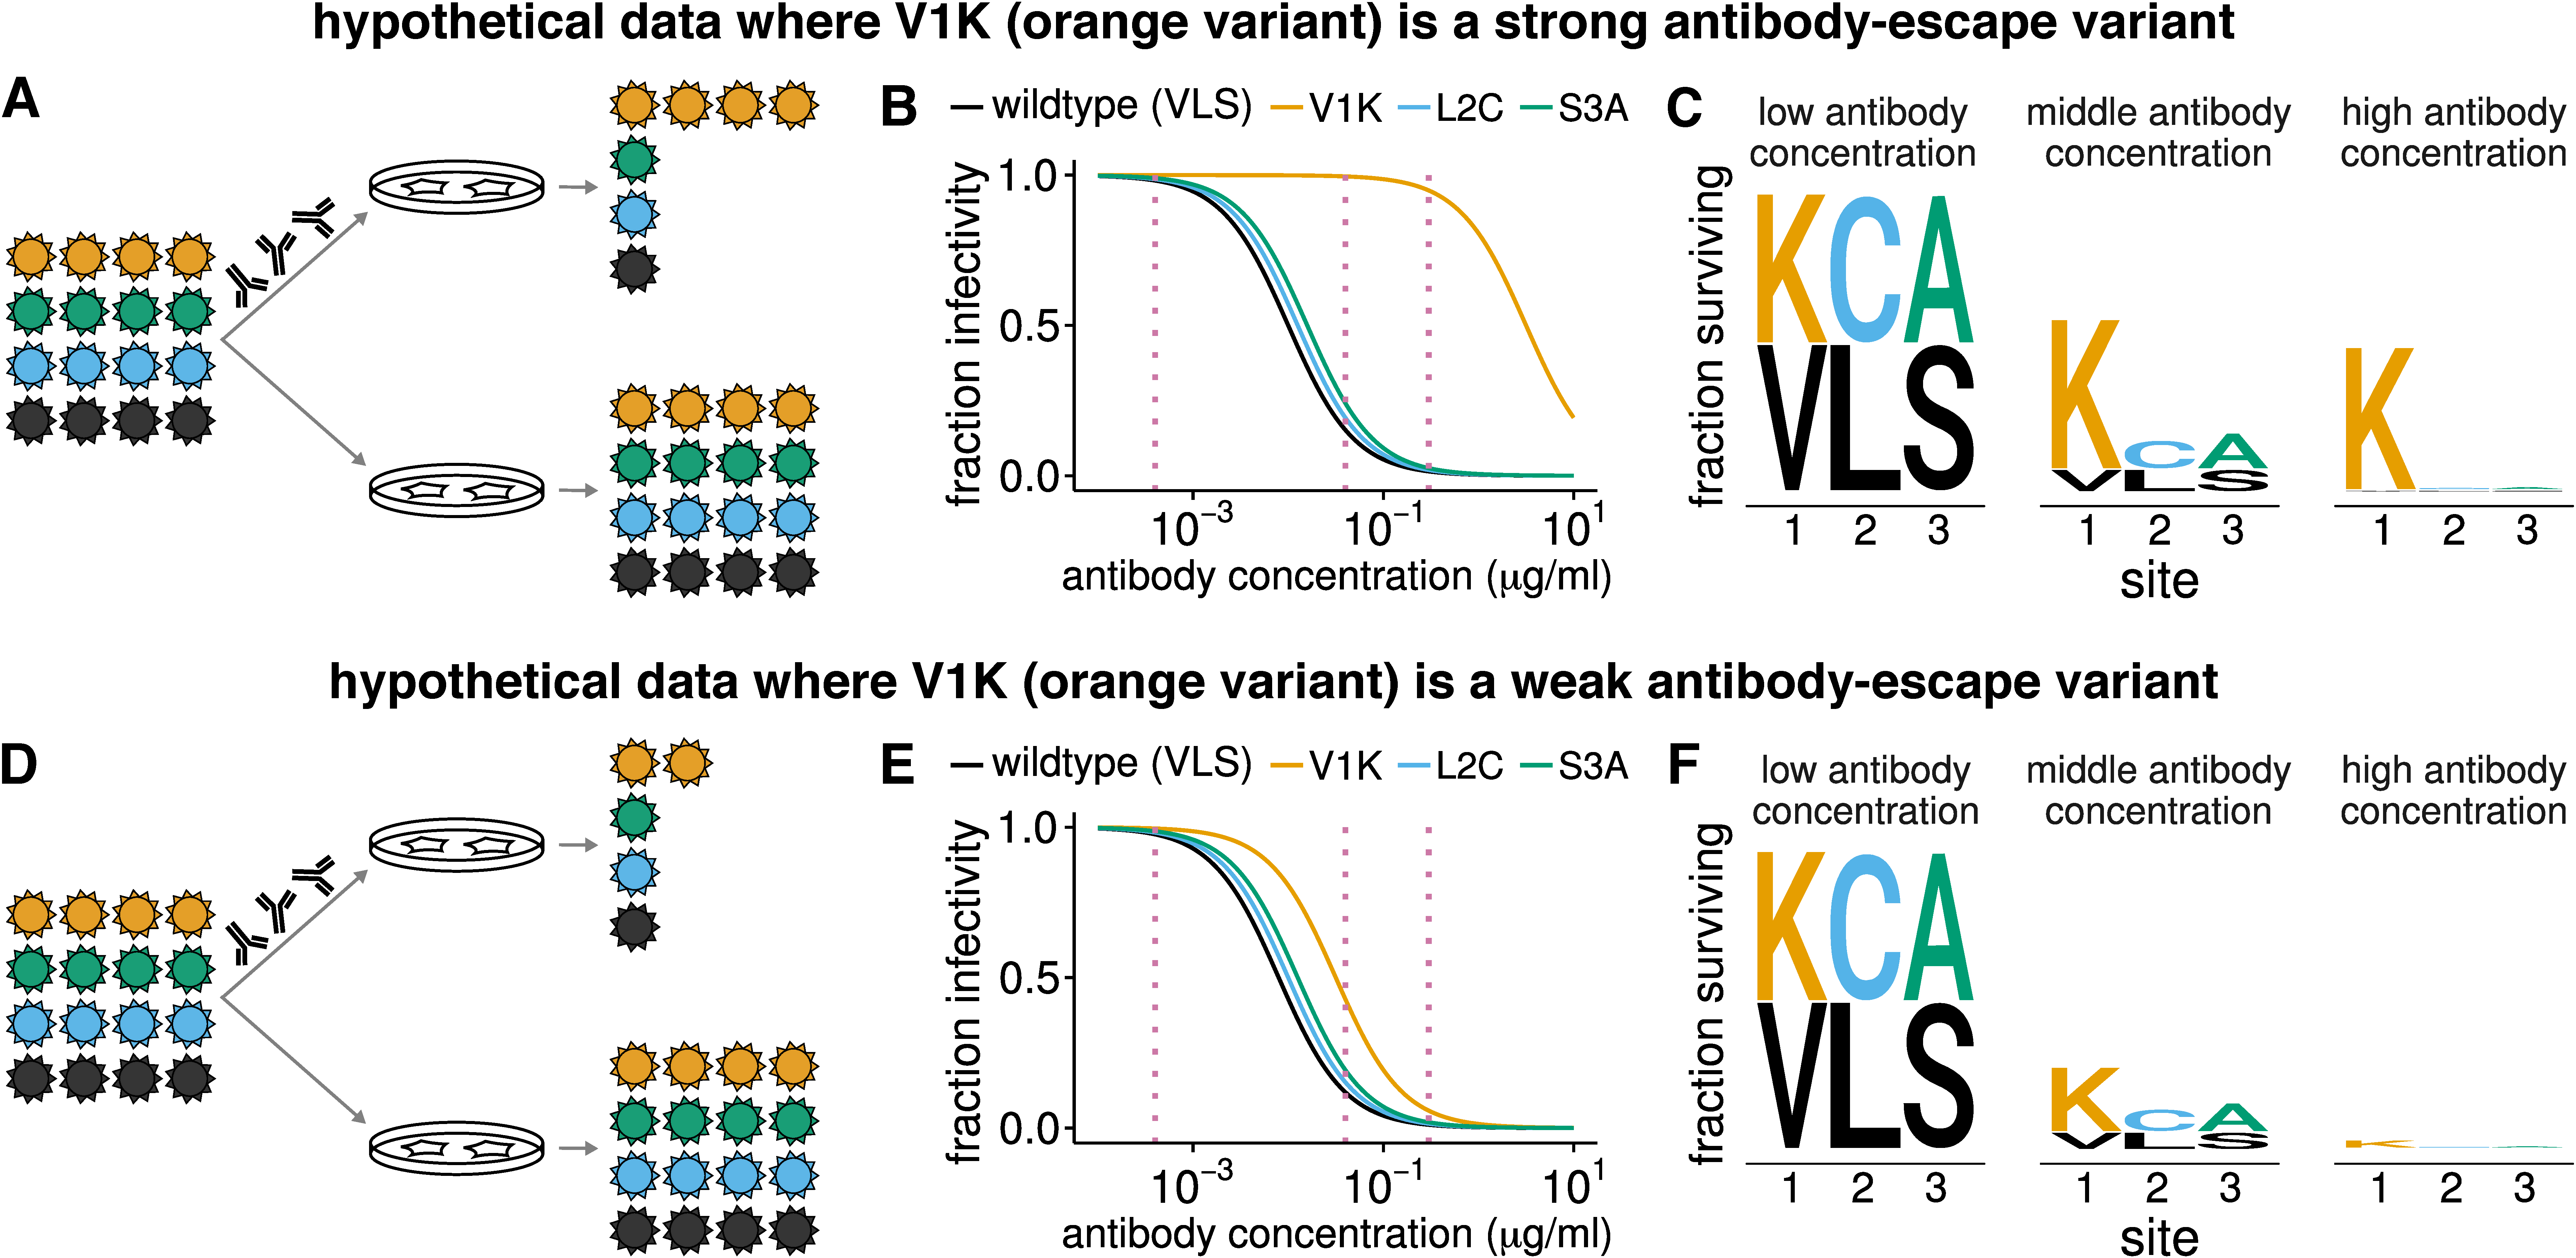
\includegraphics[width=\textwidth]{figs/fracsurvive_example/fracsurvive_fig.pdf}}
\caption{\label{fig:fracsurvive_example}
{\bf Quantifying the fraction of virions with each mutation that escape antibody neutralization.}
This figure shows hypothetical data for four viral variants.
(A) Virions with the V1K mutation (orange) completely survive an antibody concentration where most other virions are neutralized.
(B) This resistance is manifested by a large shift in V1K's neutralization curve.
(C) For each dotted vertical line drawn through the neutralization curves in (B), we calculate the fraction of virions with that mutation that survive the antibody, and indicate this fraction by the height of the letter corresponding to that amino acid at that site.
(D-F) Similar data to the first three panels, but now V1K has only a small antigenic effect, and so only modestly increases the fraction of virions that survive antibody treatment.
}
\end{figure}

Now consider the case where a mutation has just a small antigenic effect, and so only slightly increases the fraction of virions that survive neutralization (Figure~\ref{fig:fracsurvive_example}D).
In this scenario, the neutralization curve shifts only slightly (Figure~\ref{fig:fracsurvive_example}E).
In the logo plot representation, the antigenic mutation is only slightly larger than other amino acids (Figure~\ref{fig:fracsurvive_example}F), since possessing the mutation only modestly increases the chance that a virion survives antibody treatment.
These logo plots therefore provide a way to both identify antigenic mutations and quantify the magnitudes of their effects in a way that is directly comparable across antibodies.

Our goal is to determine the fraction of mutant virions that survive antibody neutralization for \emph{all} mutations to HA.
One way to do this would be to measure individual neutralization curves for each of the $19\times565 = 10,735$ single amino-acid mutants of the 565-residue HA protein.
However, individually creating and assaying that many mutants would be exceedingly time-consuming and expensive.
Fortunately, we have shown that antibody selection on all viral mutations can be assayed in a single experiment using mutational antigenic profiling~\citep{doud2017complete,dingens2017comprehensive}.
This approach involves generating viral libraries containing all mutations to the protein of interest, selecting these viruses with or without antibody, and using an accurate deep-sequencing method to determine the relative frequencies of each mutation.

These frequencies can be analyzed to calculate the fraction of virions with each mutation that survive antibody treatment.
Specifically, the deep sequencing determines the frequencies of virions carrying amino-acid $a$ at site $r$ in the antibody-selected and mock-selected conditions, which we denote as $\rho_{r,a}^{\rm{selected}}$ and $\rho_{r,a}^{\rm{mock}}$, respectively.
We can also measure the total fraction of the viral library that survives the antibody, which we denote as $\gamma$.
The fraction of variants with amino-acid $a$ at site $r$ that survive antibody selection is then simply 
\begin{equation}
\label{eq:fracsurvive}
F_{r,a} = \gamma \times \frac{\rho_{r,a}^{\rm{selected}}}{\rho_{r,a}^{\rm{mock}}}.
\end{equation}
For instance, in Figure~\ref{fig:fracsurvive_example}A, the frequency of virions with the orange mutation is $\rho_{r,a}^{\rm{selected}} = \frac{4}{7}$ in the antibody selection and $\rho_{r,a}^{\rm{mock}} = \frac{4}{16}$ in the mock selection.
The overall fraction of virions that survive the antibody in Figure~\ref{fig:fracsurvive_example}A is $\gamma = \frac{7}{16}$.
Therefore, we use Equation~\ref{eq:fracsurvive} to calculate that the fraction of variants with the orange mutation that survive is $F_{r,a} = \frac{7}{16} \times \frac{4/7}{4/16} = 1$.
Performing the analogous calculation for Figure~\ref{fig:fracsurvive_example}D correctly determines that fraction of virions with the orange mutation that survive the antibody is only 0.5 for the scenario in that figure panel.
In the analyses of real data below, we will plot the excess fraction surviving \emph{above} the overall library average, which is
\begin{equation}
\label{eq:fracsurvive_excess}
F_{r,a}^{\rm{excess}} = \max\left(0, F_{r,a} - \gamma\right).
\end{equation}
%We plot the excess fraction above the library average since this quantity more clearly accentuates antigenic mutations against the background of other mutations.
Details of how the calculations are extended to account for sequencing errors and sampling statistics are in the \nameref{sec:methods}.
Open-source software that performs all steps in the analysis beginning with the deep sequencing data is available at \url{https://jbloomlab.github.io/dms_tools2/}.

\begin{figure}
\centerline{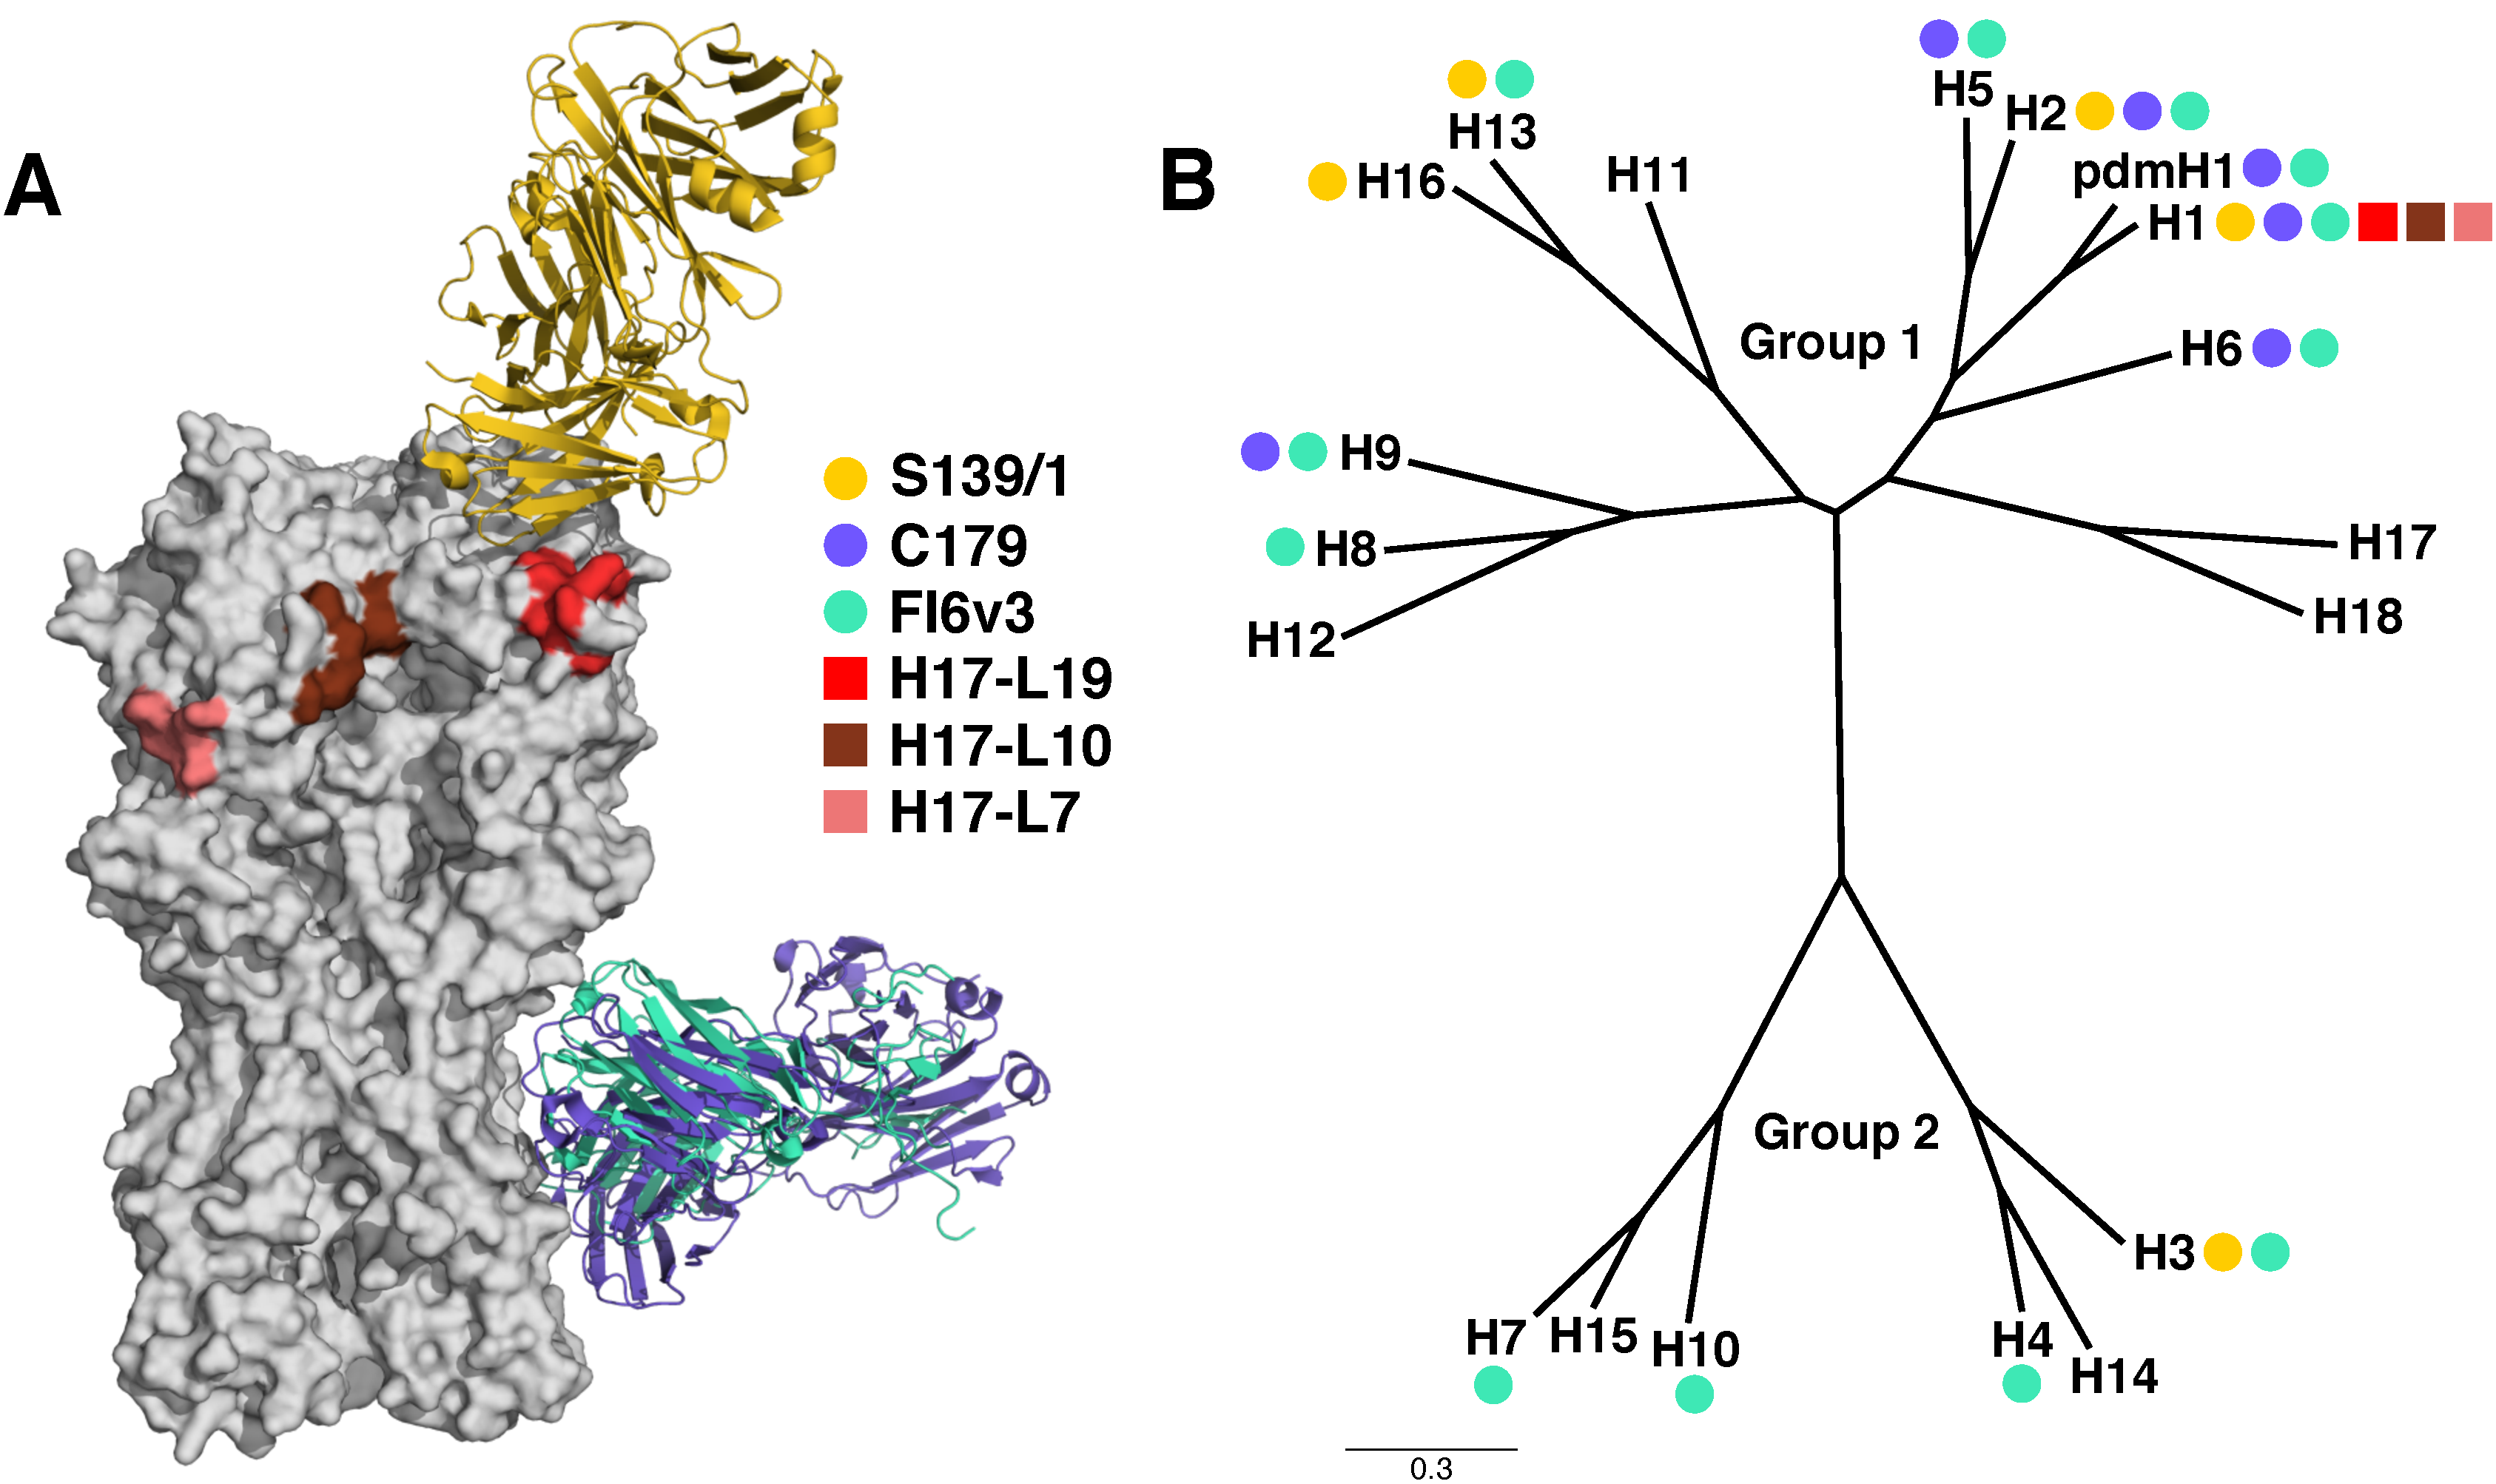
\includegraphics[width=\textwidth]{figs/antibody_summary_fig/Ab_summary.pdf}}
\caption{\label{fig:antibody_summary}
{\bf Epitopes and breadth of broad and narrow antibodies targeting HA.}
(A) Crystal structures of the broad antibodies and binding footprints of the narrow ones are superimposed on the structure of the HA trimer~\citep[PDB 1RVX;][]{gamblin2004structure}. 
S139/1~\citep[PDB 4GMS;][]{lee2012heterosubtypic} targets the receptor-binding site; C179~\citep[PDB 4HLZ;][]{dreyfus2013structure} and FI6v3~\citep[PDB 3ZTN;][]{corti2011neutralizing} target the stalk. 
The footprints for H17-L19, H17-L10, and H17-L7 are those mapped by \citet{doud2017complete}. 
(B) A phylogenetic tree of HA subtypes, with group 1 at top and group 2 at bottom.
Circles (broad antibodies) and squares (narrow antibodies) denote reported antibody binding or neutralization activity against that subtype. 
Not all antibodies have been tested against all subtypes. 
}
\end{figure}

\subsection*{Broad and narrow antibodies that neutralize influenza virus}
We applied our approach to anti-HA antibodies with a range of breadths and epitopes.
The crystal structures or binding footprints of these antibodies are shown in Figure~\ref{fig:antibody_summary}A.
We selected two broad antibodies, FI6v3 and C179, that target the stalk of HA~\citep{corti2011neutralizing, okuno1993common, dreyfus2013structure}. 
FI6v3 is extremely broad, and neutralizes both group 1 and group 2 HAs (Figure~\ref{fig:antibody_summary}B).
C179 is less broad, and neutralizes only some group 1 HAs (Figure~\ref{fig:antibody_summary}B).
We also selected a broad antibody, S139/1, that targets HA's receptor-binding site and can neutralize both group 1 and group 2 HAs~\citep{yoshida2009cross, lee2012heterosubtypic}.
Finally, we re-analyzed deep sequencing data from prior mutational antigenic profiling of three narrow strain-specific antibodies, H17-L19, H17-L10, and H17-L7~\citep{doud2017complete}.
These narrow antibodies bind the Ca2, Ca1, and Cb antigenic regions on HA's globular head~\citep{caton1982antigenic}, and only neutralize a narrow slice of H1 viruses.

We performed our experiments using the A/WSN/1933 (H1N1) strain of influenza, which is neutralized by all six antibodies with similar potencies (Figure~\ref{fig:neutcurves}).
We used antibody concentrations where nearly all wildtype virus was neutralized, allowing us to detect antigenic mutations that increase the fraction of virions that survive beyond the baseline of wildtype (Figure~\ref{fig:neutcurves}). 
We used several concentrations of each broad antibody to increase sensitivity to antigenic mutations of both large and small effect.

\begin{figure}
\centerline{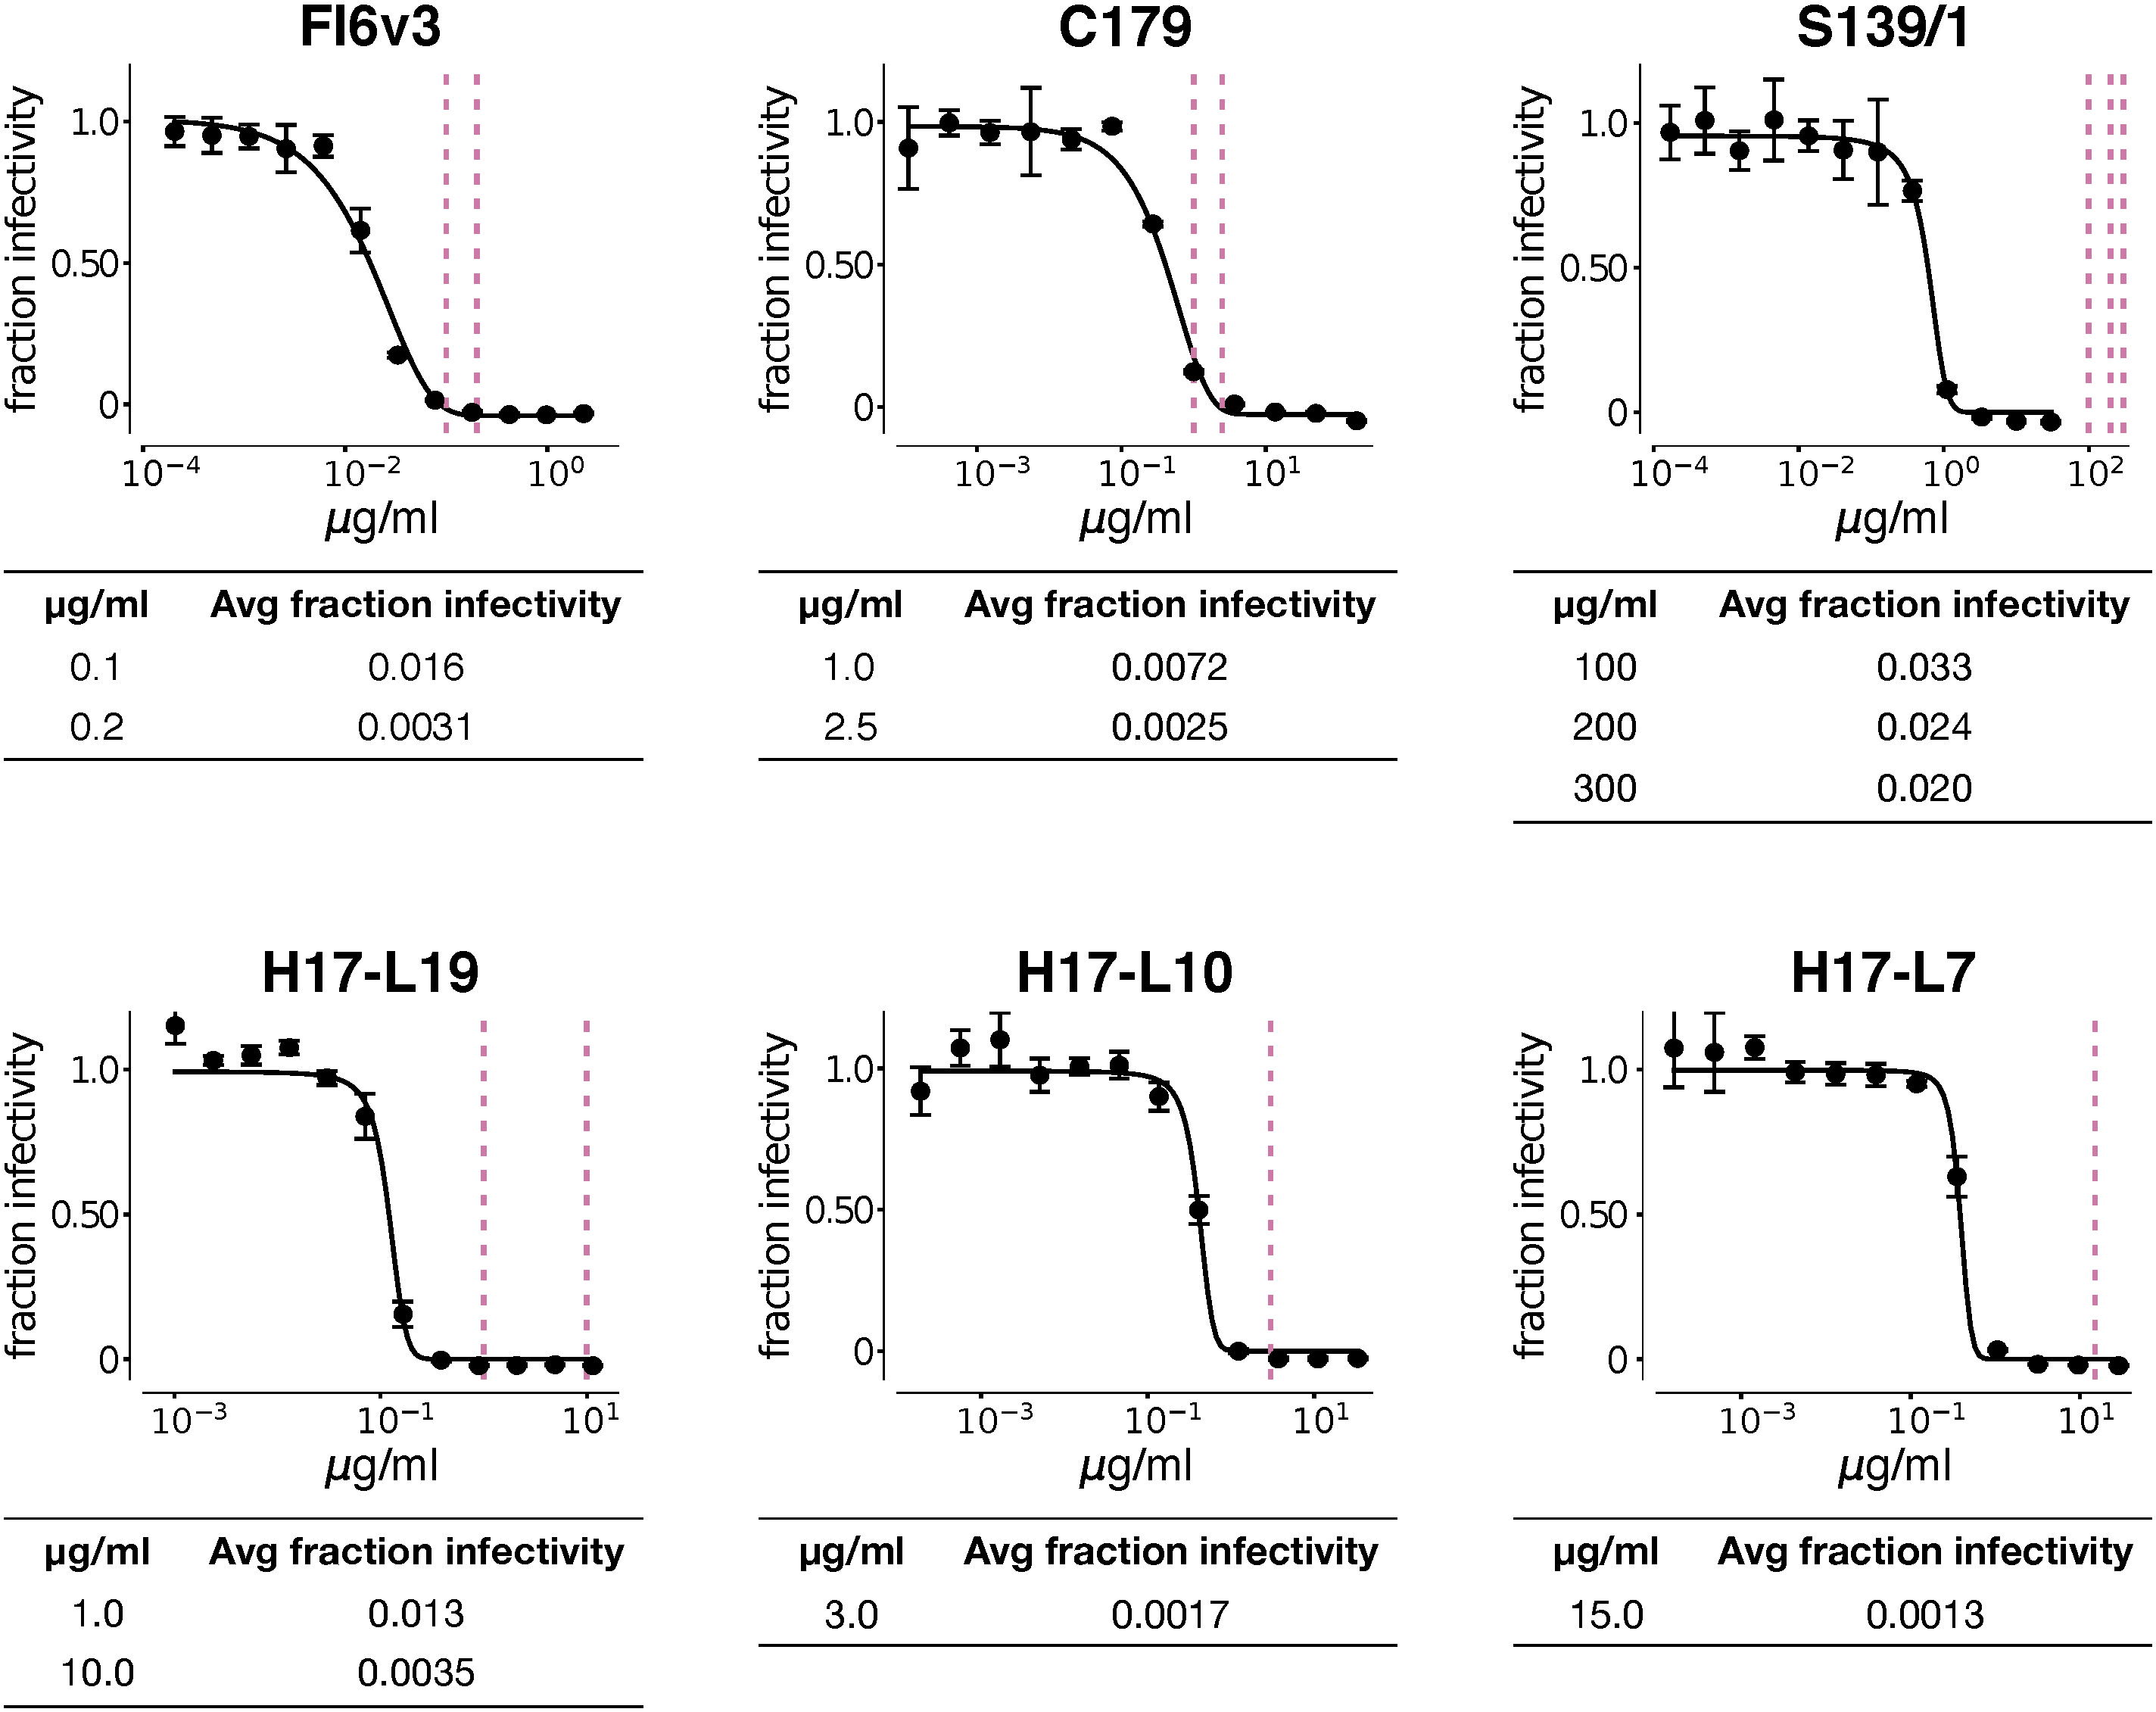
\includegraphics[width=0.8\textwidth]{figs/neutralization_curves/WT_neutralization_curves.pdf}}
\caption{\label{fig:neutcurves}
{\bf Neutralization of wildtype virus by each antibody, and the fraction of virions surviving at each concentration used in our experiments.}
The curves show neutralization of wildtype A/WSN/1933 virus. 
Each point represents the mean and standard deviation of three measurements. 
The vertical dotted lines show the concentrations of antibody used in our selections, and the tables give the overall fraction of the mutant virus libraries that survived at each concentration.
}
\end{figure}

\begin{figure}
\centerline{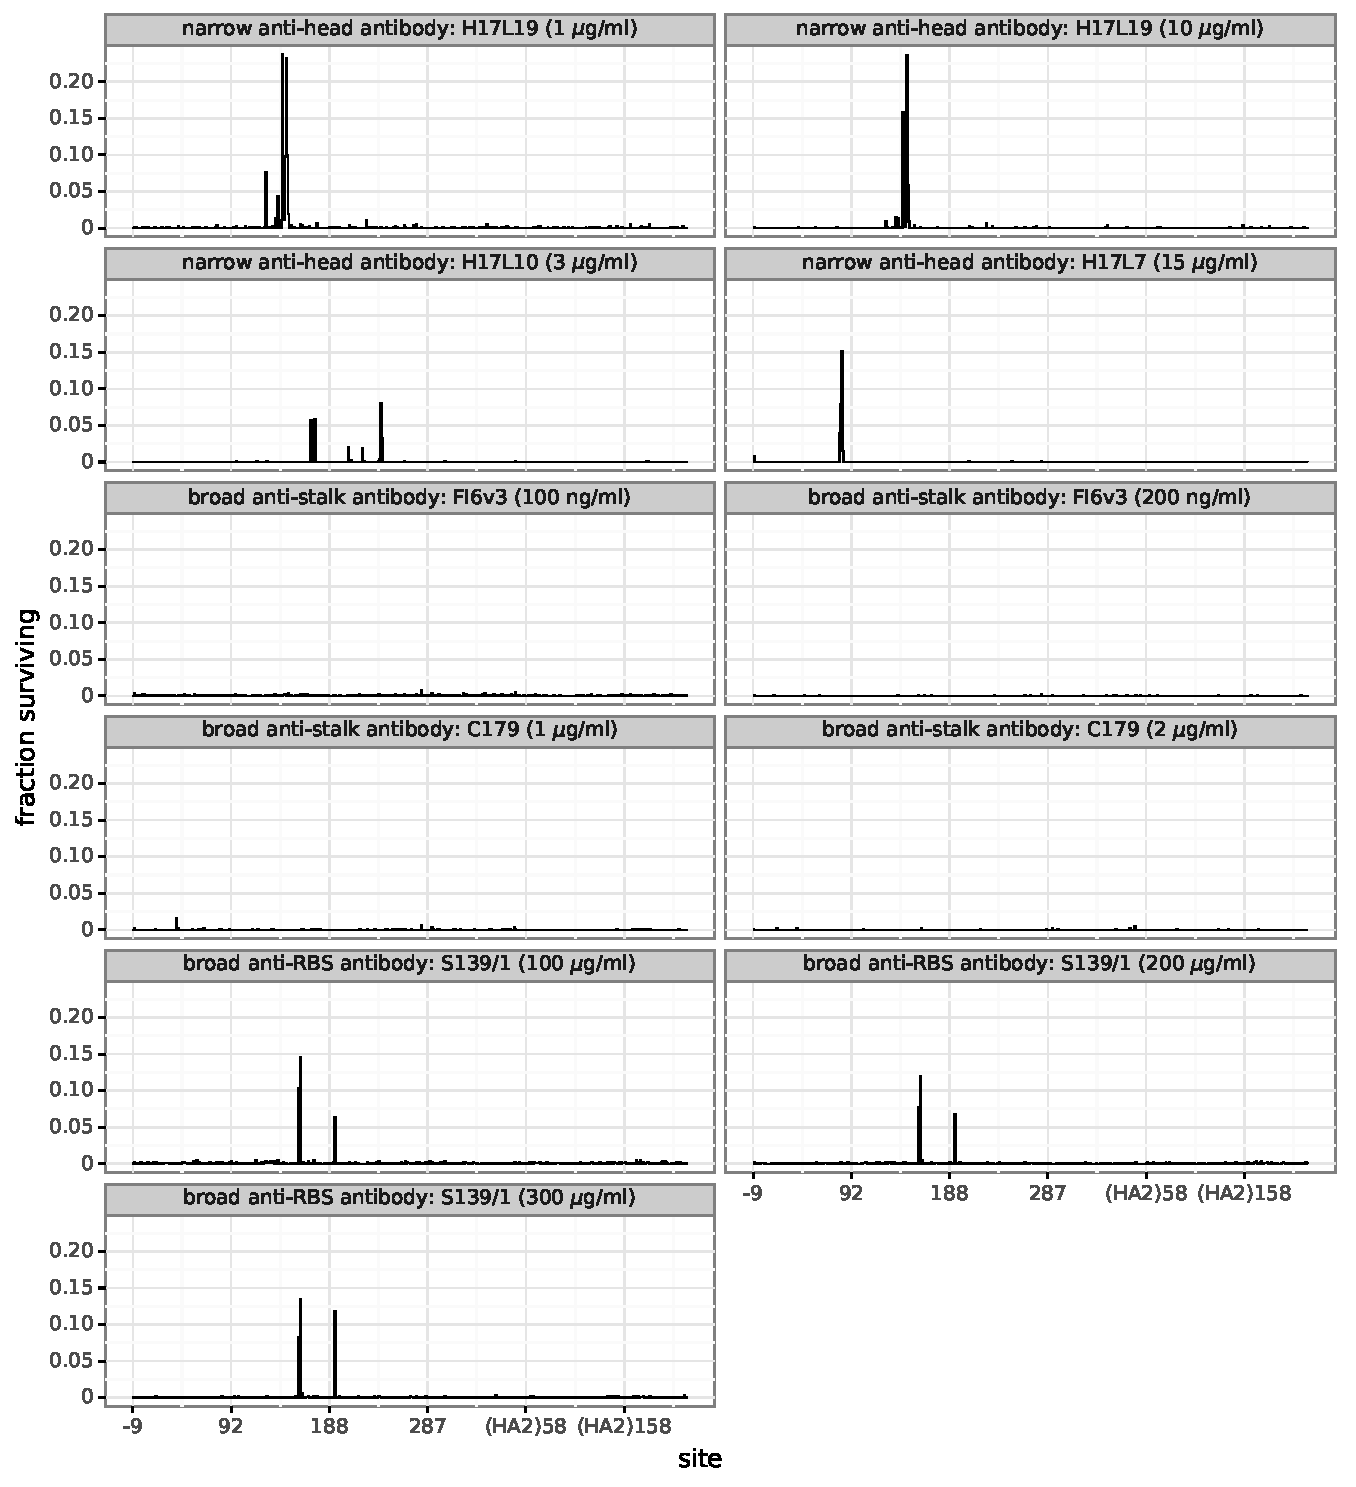
\includegraphics[width=\textwidth]{figs/avgfracsurvive.pdf}}
\caption{
\label{fig:avgfracsurvive}
{\bf Strain-specific and anti-receptor-binding-site antibodies select mutations with large antigenic effects, but anti-stalk antibodies only select small-effect mutations.}
The excess fraction of virions with a mutation at each site that survive the antibody, averaging across all amino-acid mutations at each site (see Equation~\ref{eq:avgfracsurvive}).
There are multiple sites of large-effect mutations for H17L19, H17L10, H17L7, and S139/1 -- but none for FI6v3 and C179.
Figure~\ref{suppfig:maxfracsurvive} shows the excess fraction surviving for the largest-effect mutation at each site.
Figures~\ref{suppfig:H17L19logo}, \ref{suppfig:H17L10logo}, \ref{suppfig:H17L7logo}, \ref{suppfig:FI6v3logo}, \ref{suppfig:C179logo}, and \ref{suppfig:S139logo} show all mutations using logo plots.
Sites are labeled in H3 numbering.
}
\end{figure}

\subsection*{Quantifying the antigenic effects of all mutations selected by each antibody}
We performed mutational antigenic profiling using the three broad antibodies at the concentrations indicated in Figure~\ref{fig:neutcurves}, and calculated the fraction of virions carrying each mutation that survived neutralization. 
All experiments were performed in full biological triplicate using three independently generated virus libraries carrying all single amino-acid mutations to HA~\citep{doud2016accurate}.
%We have previously described~\citep{doud2017complete} mutational antigenic profiling of the three narrow strain-specific antibodies, and we re-analyzed those deep sequencing data to calculate the fraction of virions with each mutation that survived neutralization.
The correlations among replicates are in Figure~\ref{suppfig:corr}.
For the remainder of this paper, we will refer to the median antigenic effect of each mutation across replicates.

It is immediately obvious that the narrow strain-specific antibodies and the antibody targeting HA's receptor-binding pocket (S139/1) select mutations with large antigenic effects.
For all four of these antibodies, there are multiple sites in HA where mutations enable a substantial fraction of virions to survive high antibody concentrations (Figure~\ref{fig:avgfracsurvive}).
Specifically, there are mutations that enable over a third of virions to survive at concentrations where virtually all wildtype virions are neutralized (Figure~\ref{suppfig:maxfracsurvive}).
Therefore, the virus can escape these four antibodies with the sort of large-effect single amino-acid mutations that characterize traditional influenza antigenic drift~\citep{yewdell1979antigenic,webster1980determination,koel2013substitutions,chambers2015identification,petrie2016antibodies,neher2016prediction}.  

In contrast, the stalk-targeting antibodies C179 and FI6v3 select no strong escape mutants. 
If we look at the results for these antibodies on the same scale as the other antibodies, we see only a few small bumps in the fraction of virions surviving (Figures~\ref{fig:avgfracsurvive} and \ref{suppfig:maxfracsurvive}).
Only if we zoom in can we see that there are actually a few sites where mutations slightly increase the fraction of virions surviving C179 and FI6v3 (Figures~\ref{suppfig:H17L19logo}, \ref{suppfig:H17L10logo}, \ref{suppfig:H17L7logo}, \ref{suppfig:FI6v3logo}, \ref{suppfig:C179logo}, and \ref{suppfig:S139logo}).
But the effect sizes of these antigenic mutations are tiny compared to the other antibodies -- especially for FI6v3.
Therefore, the HA of A/WSN/1933 influenza virus is far less capable of escaping these anti-stalk antibodies by single mutations than it is of escaping the other four antibodies. 

\subsection*{The selected mutations are near the binding footprints of the antibodies}
Antigenic mutations selected by narrow strain-specific antibodies against HA generally occur at residues in or near the physical binding footprint of the antibody~\citep{yewdell1979antigenic,webster1980determination,caton1982antigenic}.
We examined whether this was also the case for the broad antibodies used in our experiments.
Figure~\ref{fig:structures}A shows a zoomed-in view of the sites of mutations selected by each antibody, as well as their locations on HA's structure. 
It is immediately clear that the selected mutations are nearly all in or near the antibody-binding footprint.

\begin{figure}[h!]
\centerline{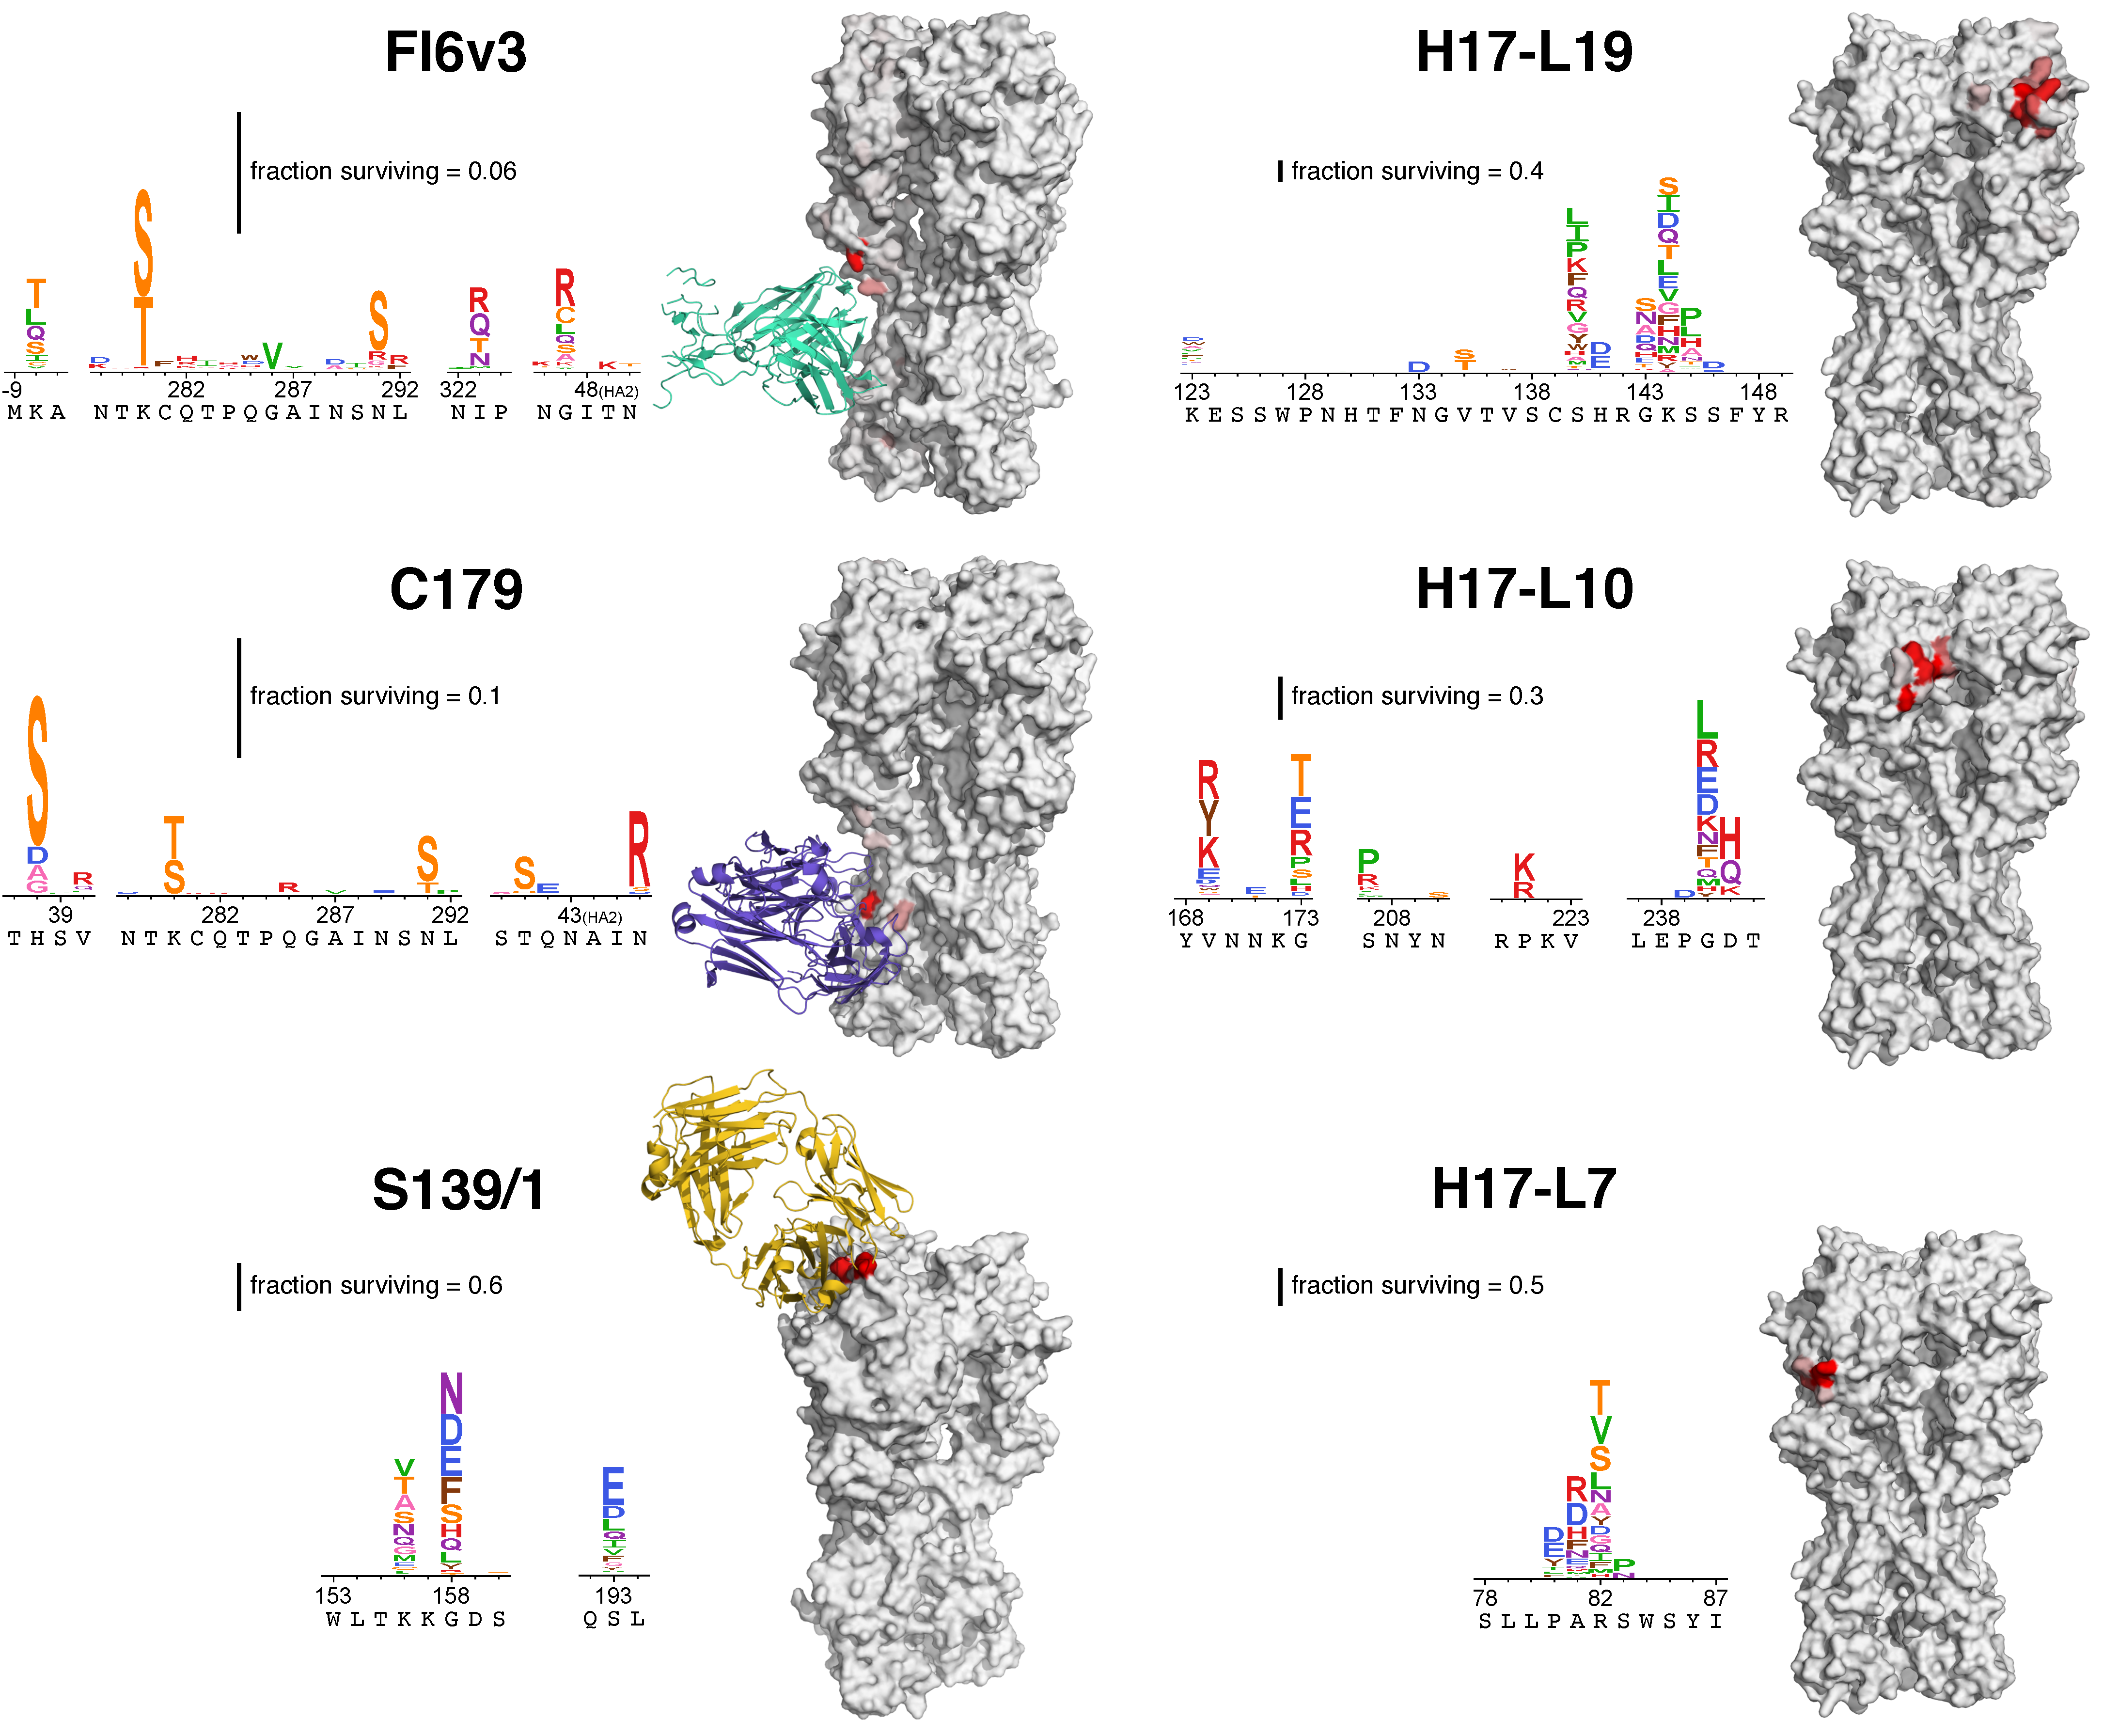
\includegraphics[width=0.89\textwidth]{figs/logoplots_pymol/logoplots_pymol.pdf}}
\caption{
\label{fig:structures}
{\bf Mutations selected by broad and narrow antibodies.}
(A) Logo plots show sites where mutations have the largest effect.
Letter heights are proportional to the excess fraction of virions with that mutation that survive antibody, as indicated by the scale bars.
Structures are colored white to red by the excess fraction surviving for the largest-effect mutation at each site, with each antibody scaled separately.  
(B) Sites of selection from anti-stalk antibodies, with the same coloring scale for both antibodies.
(C) Cladogram of HA subtypes, with group 1 in black and group 2 in gray. 
The amino acid at site 38 is indicated. 
Colors indicate whether a subtype is bound or neutralized by C179.  
}
\end{figure}

For the broad anti-receptor binding pocket antibody S139/1, we observe strong escape mutations at sites 156, 158, and 193 (Figure~\ref{fig:structures}A; sites are in H3 numbering). 
These three sites fall directly in the physical binding footprint of the antibody~\citep{lee2012heterosubtypic}, and are the same three sites where \citet{yoshida2009cross} selected escape mutants in H1, H2, and H3 HAs. 
Our data show that numerous different amino-acid mutations at each site confer neutralization resistance.
The mutation with the largest effect, D158N, introduces an N-linked glycosylation motif.

Although the anti-stalk antibodies C179 and FI6v3 only select mutations with small effects, these mutations almost all fall in the physical binding footprints of the antibodies (Figure~\ref{fig:structures}A).
The two antibodies have similar epitopes and angles of approach~\citep{dreyfus2013structure}, and they select identical mutations at several sites (Figure~\ref{fig:structures}B). 
The three largest-effect mutations for FI6v3 (K280S, K280T, and N291S) all introduce glycosylation motifs near the epitope, and all three mutations have similar magnitude antigenic effects in both FI6v3 and C179.

However, C179 selects several mutations that do not have any apparent effect on FI6v3 (Figure~\ref{fig:structures}A, Figure~\ref{suppfig:FI6v3logo}).
The most notable of these C179-specific mutations occur at site 38.
The additional breadth of FI6v3 over antibodies such as C179 that neutralize only group 1 HAs is because FI6v3 can accommodate a glycan on the asparagine at site 38 that is present in group 2 HAs~\citep{corti2011neutralizing,sui2009structural,ekiert2009antibody}. 
However, the H38S mutation that has the largest effect on C179 resistance in our experiments does not introduce a glycosylation motif, showing that there are also other ways to escape anti-stalk antibodies at this site.
Interestingly, group 1 HA subtypes that are susceptible by C179 tend to possess a histidine at site 38, but subtypes that are not bound or neutralized by C179 often possess a serine (Figure~\ref{fig:structures}C). 
%The amino-acid identity at site 111 of HA2 can change the orientation of a conserved Trp21 in HA2, also resulting in group 1 and group 2 differences in the binding ability of stalk-targeting antibodies. An H111T mutation in the A/South Carolina/1/1918 (H1N1) has been reported to abrogate C179 binding~\citep{dreyfus2013structure}.
%However, we did not observe escape mutations at site 111, but this may be due to strain-specific differences.

Interestingly, FI6v3 weakly selects several mutations at residue -8, which is part of HA's signal peptide (Figure~\ref{fig:structures}A). 
This signal peptide is cleaved from the mature HA protein~\citep{daniels2003n,burke2014recommended}, so mutations at this site may affect the density of HA trimers on the virion~\citep{nordholm2017translational} rather than the physical binding of the antibody to HA.

\subsection*{Neutralization assays validate the mutational antigenic profiling}
Do the mutations identified in our mutational antigenic profiling actually have the expected effect on antibody neutralization?
We have previously validated many of the large-effect antigenic mutations selected by the narrow antibodies H17-L19, H17-L10, and H17-L7~\citep{doud2017complete}.
However, the mutations selected by the broad anti-stalk antibodies have much smaller effects -- especially for the broadest antibody, FI6v3.
We therefore tested some of these FI6v3-selected mutations using neutralization assays on individual viral mutants.

\begin{figure}
\centerline{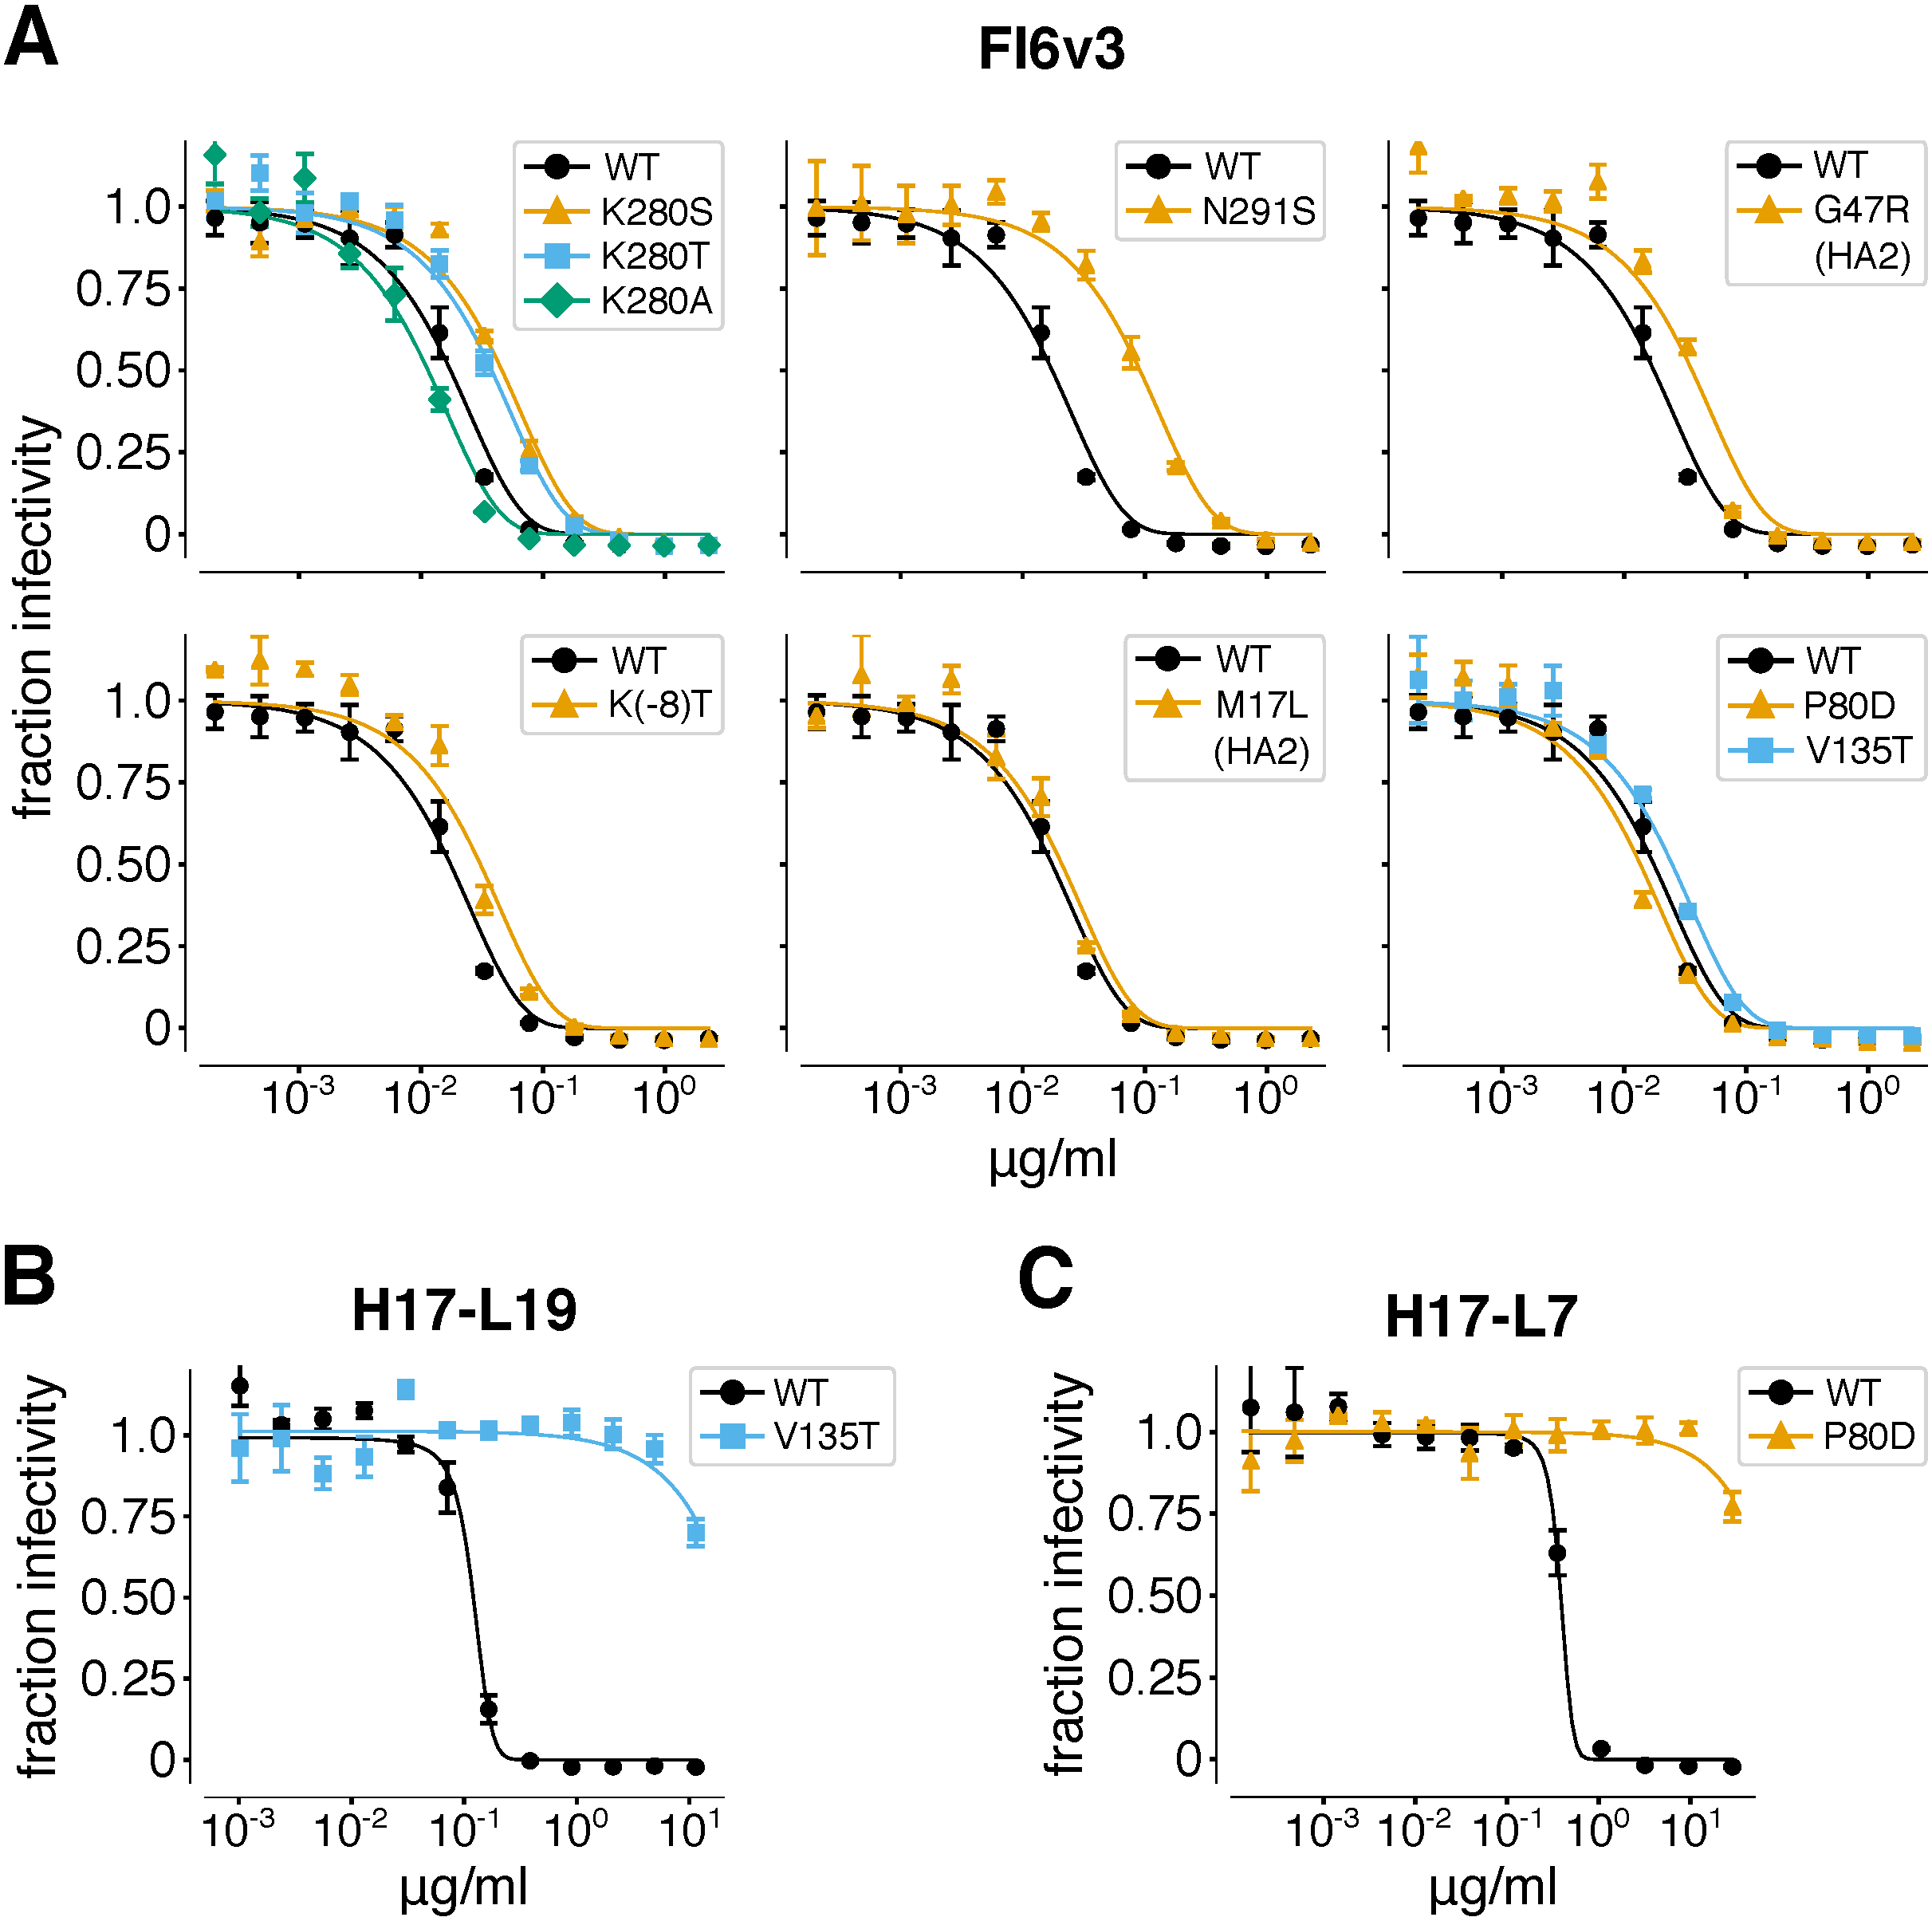
\includegraphics[width=0.8\textwidth]{figs/FI6v3mutant_neutcurves/FI6v3_mutant_neutcurves.pdf}}
\caption{
\label{fig:FI6v3neutcurves}
{\bf The mutations selected by FI6v3 increase neutralization resistance, but the effects are small.}
(A) Neutralization curves of individual viral mutants with FI6v3.
The mutations K280S, K280T, N291S, G47R (HA2), and K(-8)T are all expected to increase neutralization resistance based on the mutational antigenic profiling (Figure~\ref{fig:structures}A), and they all do so -- but only modestly. 
The mutations K280A, M17L (HA2), P80D, and V135T are \emph{not} expected to affect neutralization based on the mutational antigenic profiling (Figure~\ref{suppfig:FI6v3logo}, and none of them do.
(B), (C) In contrast to FI6v3, mutations selected by other antibodies have very large effects on neutralization.
Shown are neutralization curves for representative escape mutants from H17-L19 and H17-L7 taken from \citet{doud2017complete}; that paper also shows additional examples of large-effect escape mutations from these antibodies.
}
\end{figure}

Figure~\ref{fig:FI6v3neutcurves} shows that the mutational antigenic profiling is highly predictive of the results of the neutralization assays, even for small-effect mutations.
As discussed in the previous section, the three mutations most strongly selected by FI6v3 introduce glycosylation motifs at sites 278-280 or 289-291 (Figure~\ref{fig:structures}A).
We created viruses carrying each of these mutations (K280S, K280T, and N291S) and validated that all three mutants were modestly more resistant to FI6v3 (Figure~\ref{fig:FI6v3neutcurves}A).
As a control, we also validated that a mutation at one of these sites (K280A) that does \emph{not} have an effect in our mutational antigenic profiling does not shift the neutralization curve (Figure~\ref{fig:FI6v3neutcurves}A).
Interestingly, the HA of pandemic H1N1 has a glycosylation motif at 278-280, and \citet{corti2011neutralizing} have reported that this HA is $\sim$4-fold more resistant to FI6v3 than the A/WSN/1933 HA used in our experiments.
This reported difference between strains is of similar magnitude to the effect that we measure for introducing the glycosylation motif via the K280S or K280T mutations.

Our mutational antigenic profiling also identified several non-glycosylation-motif mutations that were selected by FI6v3.
We validated that one of these mutations, G47R in the HA2 chain, indeed increased neutralization resistance (Figure~\ref{fig:FI6v3neutcurves}A) -- although as predicted by the mutational antigenic profiling, the magnitude of the effect was smaller than for the glycosylation-motif mutations.
The most unexpected mutations identified in the mutational antigenic profiling were at site -8 in the signal peptide.
We tested one of these mutations, K(-8)T, and found that it indeed caused a modest but detectable increase in neutralization resistance (Figure~\ref{fig:FI6v3neutcurves}A).
As controls, we also tested three more mutations (P80D, V135T, and M17L in HA2) that did \emph{not} have substantial effects in the mutational antigenic profiling, and confirmed that none of them affected neutralization resistance.

A remarkable aspect of these validation experiments is the very small effect sizes of the identified mutations.
Antigenic mutations selected by strain-specific antibodies to HA generally increase the concentration of antibody needed to neutralize the virus by orders of magnitude.
Neutralization curves for a few examples of such large-effect escape mutants are in Figure~\ref{fig:FI6v3neutcurves}B,C.
Our work demonstrates that there are no such large-effect single mutations to the A/WSN/1933 HA when it comes to escaping from FI6v3 and C179.
But the results in Figure~\ref{fig:FI6v3neutcurves}A show that we can still leverage the high sensitivity of mutational antigenic profiling to identify mutations that have much more modest but nonetheless measurable effects on antibody neutralization.

\section*{DISCUSSION}
Some discussion

\clearpage
\small

\section*{METHODS}
\label{sec:methods}
\subsection*{Antibodies}
FI6v3 was expressed and purified by the Fred Hutchinson Cancer Research Center protein expression core \comment{i think?}.
C179 was purchased from Takara Bio Inc (Catalog \# M145).
S139/1 heavy and light chain variable sequences were obtained from PDB ID 4GMS~\cite{lee2012heterosubtypic} and expressed and purified by the Fred Hutchinson Cancer Research Center protein expression core.

\subsection*{Neutralization assays}
We performed neutralization assays as previously described in~\citep{hooper2013mutant} using WSN GFP reporter viruses. Viruses carrying GFP in the PB1 segment were grown using reverse genetics plasmids in complementing 293T-CMV-PB1 and MDCK-SIAT1-CMV-PB1 cells that constitutively express the PB1 protein. 

\subsection*{Mutant virus selections with antibody and deep sequencing}
Library selections and deep sequencing were performed as previously described in~\cite{doud2017complete}. 
We conducted the antibody selections using the mutant virus libraries from~\cite{doud2016accurate}. 
We diluted the virus libraries to a concentration of $1 \times 10^{6}$ TCID$_{50}$ per ml and incubated the virus dilutions with an equal volume of antibody at the intended concentration.
We then incubated the virus-antibody mixture at 37$^\circ$C for 1.5 hours
Each selection was done in biological triplicate at the antibody concentrations shown in Figure~\ref{fig:neutcurves} concentrations, and technical replicates of some of the concentrations were also performed. 
To estimate the fraction of the overall library surviving selection, denoted as $\gamma$ in this paper, we made duplicate 10-fold serial dilutions of each of the virus libraries to use as a standard curve of infectivity. 
qRT-PCR of the standard curves were performed as previously described in~\cite{doud2017complete} using qPCR primers for WSN influenza nucleoprotein (NP) to quantify viral infectivity and primers for canine GAPDH to correct for RNA amounts.
Next, we fit a linear regression of the log(infectious dose) versus the mean difference in qPCR Ct values between NP and GAPDH to estimate the total library fraction infectivity after antibody selection.

\subsection*{Construction of HA phylogenetic tree}
We downloaded one HA sequence per subtype from the NIAID Influenza Research Database (IRD) \comment{cite}, built the phylogenetic tree using RaxML \comment{cite}, and visualized the tree using FigTree \comment{cite}. The HA sequences we downloaded were: H1 (A/WSN/1933); pdmH1N1 (A/California/04/2009); H2 (A/Japan/305/1957); H3 (A/Aichi/2/1968); H4 (A/swine/Ontario/01911/2/1999); H5 (A/Vietnam/1203/2004); H6 (A/chicken/Taiwan/0705/1999); H7 (A/Netherlands/219/2003); H8 (A/turkey/Ontario/6118/1968); H9 (A/swine/HongKong/9/1998); H10 (A/mallard/Bavaria/3/2006); H11 (A/duck/England/1/1956); H12 (A/duck/Alberta/60/1976); H13 (A/gull/Maryland/704/1977); H14 (A/mallard/Astrakhan/263/1982); H15 (A/mallard duck/Sweden/139579/2012); H16 (A/black headed gull/Mongolia/1756/2006); H17 (A/little yellow-shouldered bat/Guatemala/060/2010); H18 (A/dark fruit-eating bat/Bolivia/PBV780-781/2011).

For the cladogram in Figure~\ref{fig:structures}C, the amino-acid identities at site 38 are from the strains tested against C179 in~\cite{dreyfus2013structure}. For subtypes not tested, we used the identity from the corresponding strain listed above.

We denoted HA's with reported binding or neutralization activity by each antibody, and defined binding activity as \comment{binding to full influenza virus, VLPs, recombinant or purified HA's}. Among broad antibodies, S139/1 has not been tested against H8, H9, and H11; C179 has not been tested against H8 and H11; no antibodies have been tested against H17 and H18.

\subsection*{H3 sequence numbering}
Unless otherwise indicated, all residues are numbered in H3 numbering in this paper, with the signal peptide in negative numbers, the HA1 subunit as plain numbers, and the HA2 subunit denoted with "(HA2)". We converted the sequential residue numbers into H3 numbering by running the Python script available on \url{https://github.com/jbloomlab/HA_numbering}. In this script, we used MUSCLE to align the WSN/1933 H1 HA sequence to the 4HMG pdb sequence for the A/Aichi/2/1968 H3 HA \comment{cite Weis1990JMB}, which allowed us to convert from the sequential numbering to the H3 numbering scheme. 

\subsection*{Calculating the fraction of virions with each mutation that escapes antibody neutralization}
In prior mutational antigenic profiling work~\citep{doud2017complete,dingens2017comprehensive}, we calculated the differential selection on each mutation as the logarithm of its enrichment relative to wildtype in an antibody-selected sample versus a mock-selected control.
These \emph{mutation differential selection} values are useful for the analysis of individual experiments.
However, there is no natural way to compare these values across experiments with different antibodies at different concentrations, since the strength of differential selection depends on details of how the pressure is imposed.
We therefore developed the new approach in this paper to quantify the antigenic effect of a mutation in units that can be compared across antibodies and concentrations.

The general principle of the calculations is illustrated in Figure~\ref{fig:fracsurvive_example} and discussed in the first section of the \nameref{sec:results}.
Here we provide details on how these calculations are performed.
The deep sequencing measures the number of times that codon $x$ is observed at site $r$ in both the antibody-selected and mock-selected conditions. 
Denote these counts as $n_{r,x}^{\rm{selected}}$ and $n_{r,x}^{\rm{mock}}$, respectively.
We also perform deep sequencing of a control (in this case, plasmid DNA encoding the wildtype HA gene) to estimate the sequencing error rate.
Denote the counts of codon $x$ at site $r$ in this control as $n_{r,x}^{\rm{err}}$.
Also denote the total reads at each site $r$ in each sample as
$N_{r}^{\rm{selected}} = \sum_x n_{r,x}^{\rm{selected}}$,
$N_{r}^{\rm{mock}} = \sum_x n_{r,x}^{\rm{mock}}$, and
$N_{r}^{\rm{err}} = \sum_x n_{r,x}^{\rm{err}}$.

We first estimate the rate of sequencing errors at site $r$ as
\begin{equation}
\label{eq:epsilonrx}
\epsilon_{r,x} = \frac{n_{r,x}^{\rm{err}}}{N_{r}^{\rm{err}}}.
\end{equation}
For the wildtype identity at site $r$, which we denote as $\operatorname{wt}\left(r\right)$, the value of $\epsilon_{r,\operatorname{wt}\left(r\right)}$ is the fraction of times we correctly observe the wildtype identity $\operatorname{wt}\left(r\right)$ at site $r$ versus observing some spurious mutation. 
For all mutant identities $x \ne \operatorname{wt}\left(r\right)$ at site $r$, $\epsilon_{r,x}$ is the fraction of times we observe the mutation $x$ at site $r$ when the identity is really wildtype.
We ignore second-order terms where we incorrectly read one mutation as another, as such errors will be very rare as mutations themselves are rare (most codons are wildtype in most sequences). 

We next adjust all of the deep sequencing codon counts in the antibody-selected and mock-selected conditions by the error control. 
Specifically, the error-adjusted counts for the antibody-selected sample are
\begin{equation}
\label{eq:erroradjust}
\hat{n}_{r,x} ^{\rm{selected}}= \begin{cases}
\max\left[N_r^{\rm{selected}} \times \left(\frac{n_{r,x}^{\rm{selected}}}{N_r^{\rm{selected}}} - \epsilon_{r,x}\right), 0\right] & \mbox{if } x \ne \operatorname{wt}\left(r\right) \\
n_{r,x} / \epsilon_{r,x} & \mbox{if } x = \operatorname{wt}\left(r\right).
\end{cases}
\end{equation}
An equivalent equation is used to calculate $\hat{n}_{r,x} ^{\rm{mock}}$.
We then sum the error-adjusted codon counts for each amino acid $a$:
\begin{equation}
\hat{n}_{r,a}^{\rm{selected}} = \sum\limits_{\left\{x \mid \mathcal{A}\left(x\right) = a\right\}} \hat{n}_{r,x}^{\rm{selected}},
\end{equation}
so that $\hat{n}_{r,a}^{\rm{selected}}$ are the error-adjusted counts for the antibody-selected condition summed across all codons $x$ where the encoded amino acid $\mathcal{A}\left(x\right)$ is $a$.
An equivalent equation is used to calculate $\hat{n}_{r,a} ^{\rm{mock}}$.

Finally, we use these error-adjusted amino-acid counts to estimate the mutation frequencies $\rho_{r,a}^{\rm{selected}}$ and $\rho_{r,a}^{\rm{mock}}$ that are used in Equation~\ref{eq:fracsurvive} to calculate the fraction $F_{r,a}$ of virions with amino acid $a$ at site $r$ that survive the selection.
When estimating these mutation frequencies, we add a pseudocount of $P = 5$ to the lower-depth sample, and a depth-adjusted pseudocount to the higher depth sample.
The rationale for adding a pseudocount is to regularize the estimates in the case of low counts.
Specifically, we estimate the mutation frequencies as
\begin{eqnarray}
\rho_{r,x}^{\rm{selected}} &=& \frac{n_{r,x}^{\rm{selected}} + f_{r, \rm{selected}} \times P}{N_r^{\rm{selected}} + f_{r, \rm{selected}} \times P \times A} \\
\rho_{r,x}^{\rm{mock}} &=& \frac{n_{r,x}^{\rm{mock}} + f_{r, \rm{mock}} \times P}{N_r^{\rm{mock}} + f_{r, \rm{mock}} \times P \times A} 
\end{eqnarray}
where $A$ is the number of characters (e.g., 20 for amino acids), $f_{r, \rm{selected}}$ and $f_{r, \rm{mock}}$ are the pseudocount adjustment factors defined as:
\begin{eqnarray}
f_{r, \rm{selected}} &=& \max\left(1, \frac{N_{r}^{\rm{selected}}}{N_{r}^{\rm{mock}}}\right) \\
f_{r, \rm{mock}} &=& \max\left(1, \frac{N_{r}^{\rm{mock}}}{N_{r}^{\rm{selected}}}\right).
\end{eqnarray}
The pseudocount adjustment factors ensure that $P$ is added to the counts for the lower depth sample, and a proportionally scaled-up pseudocount is added to the higher depth sample.
The depth scaling is necessary to avoid systematically biasing towards higher mutation frequencies in the lower depth sample.
It is these estimated mutation frequencies that are used in conjunction with $\gamma$ (the qPCR estimated overall of virions that survive selection) to compute the fraction surviving ($F_{r,a}$) and excess fraction surviving above the library average ($F_{r,a}^{\rm{excess}}$) via Equations~\ref{eq:fracsurvive} and \ref{eq:fracsurvive_excess}.

In some cases, we need to summarize the excess fraction of mutations surviving into a single number for each site, such as for plotting as a function of the site number or displaying on the crystal structure.
There are 19 different $F_{r,a}^{\rm{excess}}$ values for non-wildtype amino acids for each site. 
One summary statistic is the fraction surviving above the library average \emph{averaged} over all 19 amino-acid mutations at site $r$:
\begin{equation}
\label{eq:avgfracsurvive}
\mathcal{F}_r^{avg} = \frac{1}{19} \sum\limits_{\left\{a \mid a \ne \operatorname{wt}\left(r\right)\right\}} F_{r,a}^{\rm{excess}}.
\end{equation}
Another summary statistic is the \emph{maximum} fraction surviving above average among all 19 amino-acid mutations at site $r$:
\begin{equation}
\label{eq:maxfracsurvive}
\mathcal{F}_r^{max} = \frac{1}{19} \max\limits_{\left\{a \mid a \ne \operatorname{wt}\left(r\right)\right\}}\left( F_{r,a}^{\rm{excess}} \right).
\end{equation}

Code that performs all these calculations is included in the \texttt{dms\_tools2} software package~\citep{bloom2015software} which is available at \url{http://jbloomlab.github.io/dms_tools2}.
The in this paper were performed using version 2.1.0 of \texttt{dms\_tools2}.

\subsection*{Data availability and source code}
Deep sequencing data are available from the Sequence Read Archive under BioSample accession SAMN05789126.

\subsection*{ACKNOWLEDGMENTS}
This work was supported by grants R01GM102198 and R01AI127893 from the NIGMS and NIAID of the NIH.
MBD was supported in part by training grant T32AI083203 from the NIAID of the NIH.
JML was supported in part by \comment{CIDID grant}.
The research of JDB is supported in part by a Faculty Scholar Grant from the Howard Hughes Medical Institute and the Simons Foundation.

\bibliographystyle{mbe}
\bibliography{references.bib}

\clearpage
\normalsize

\section*{Supplementary Material}
\FloatBarrier
\pagenumbering{arabic}% resets `page` counter to 1
\renewcommand*{\thepage}{S\arabic{page}}

\begin{suppfigure}
\centerline{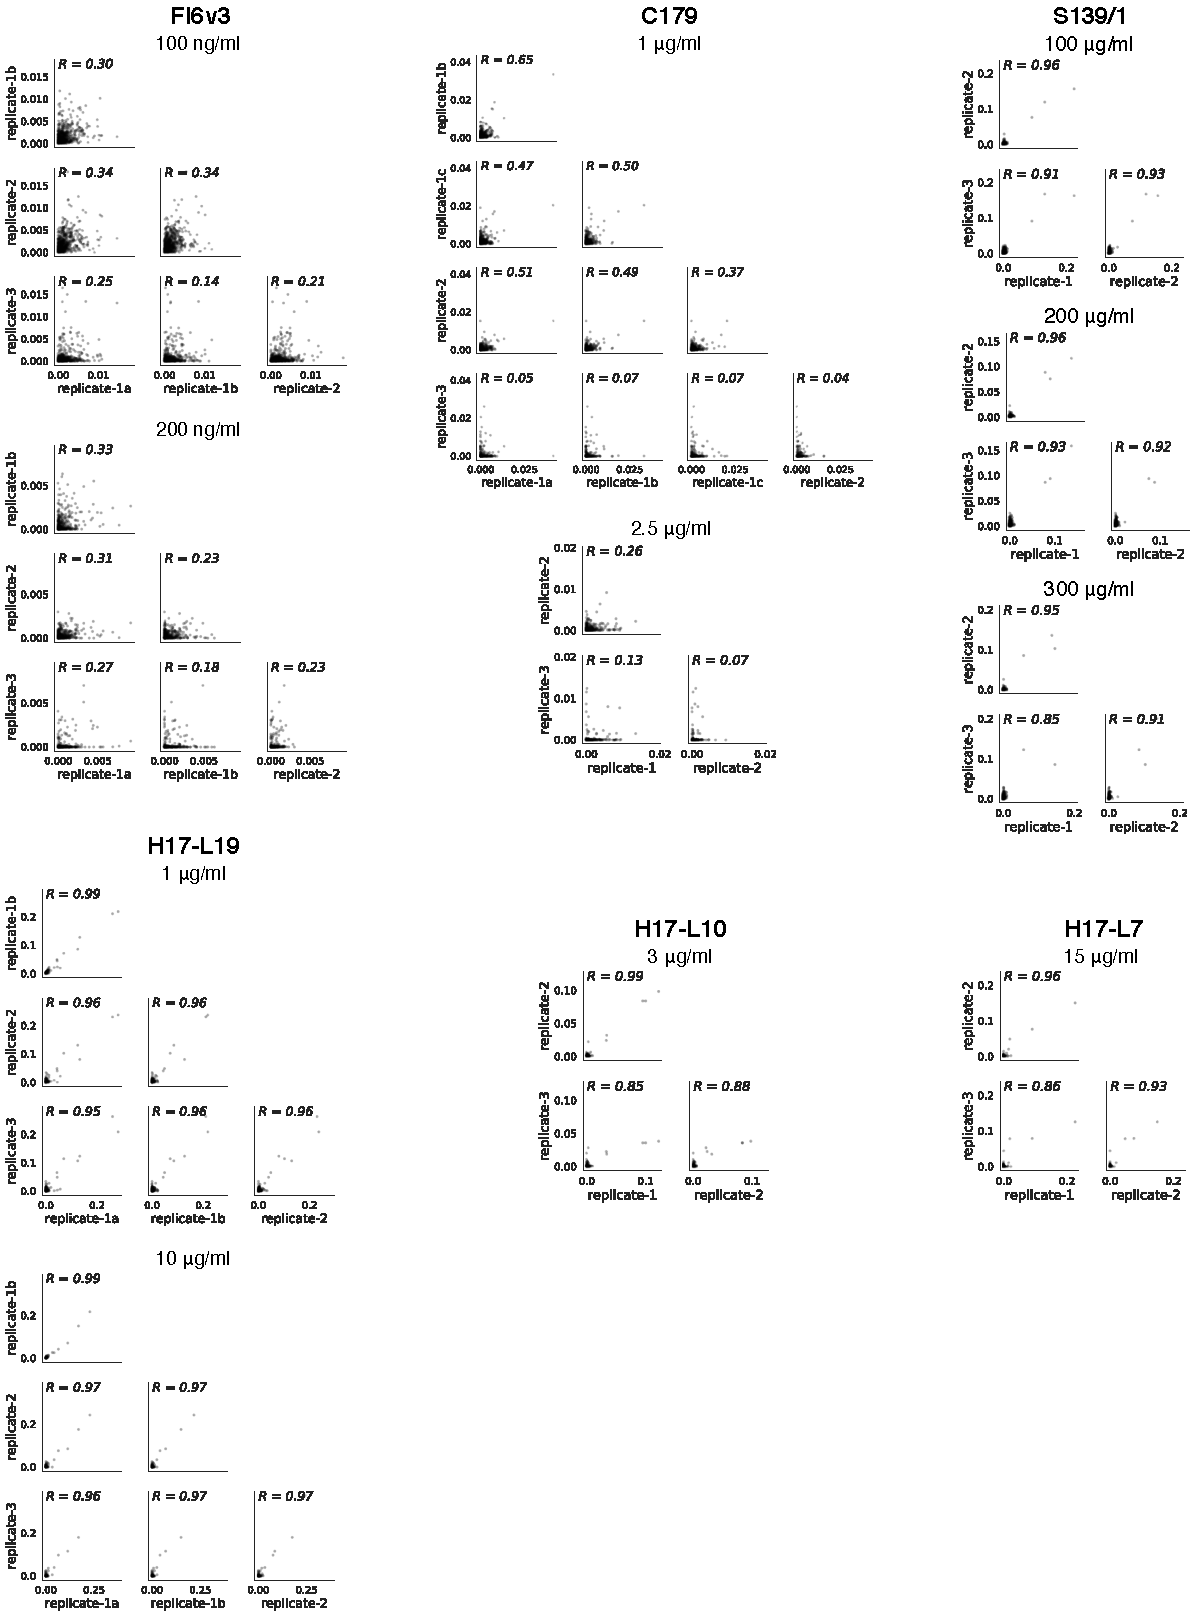
\includegraphics[width=0.84\textwidth]{figs/corrs/site_correlations.pdf}}
\caption{\label{suppfig:corr}
{\bf Correlations across experimental replicates.} 
Each point represents one site in HA, and gives the fraction surviving above average across all amino-acid mutations at that site, as calculated using Equation~\ref{eq:avgfracsurvive}.
The replicates are highly correlated for antibodies with strong escape mutations (S139/1, H17-L19, H17-L10, and H17-L7), and reasonably correlated for antibodies with only weak escape mutations (FI6v3 and C179).
}
\end{suppfigure}

\begin{suppfigure}
\centerline{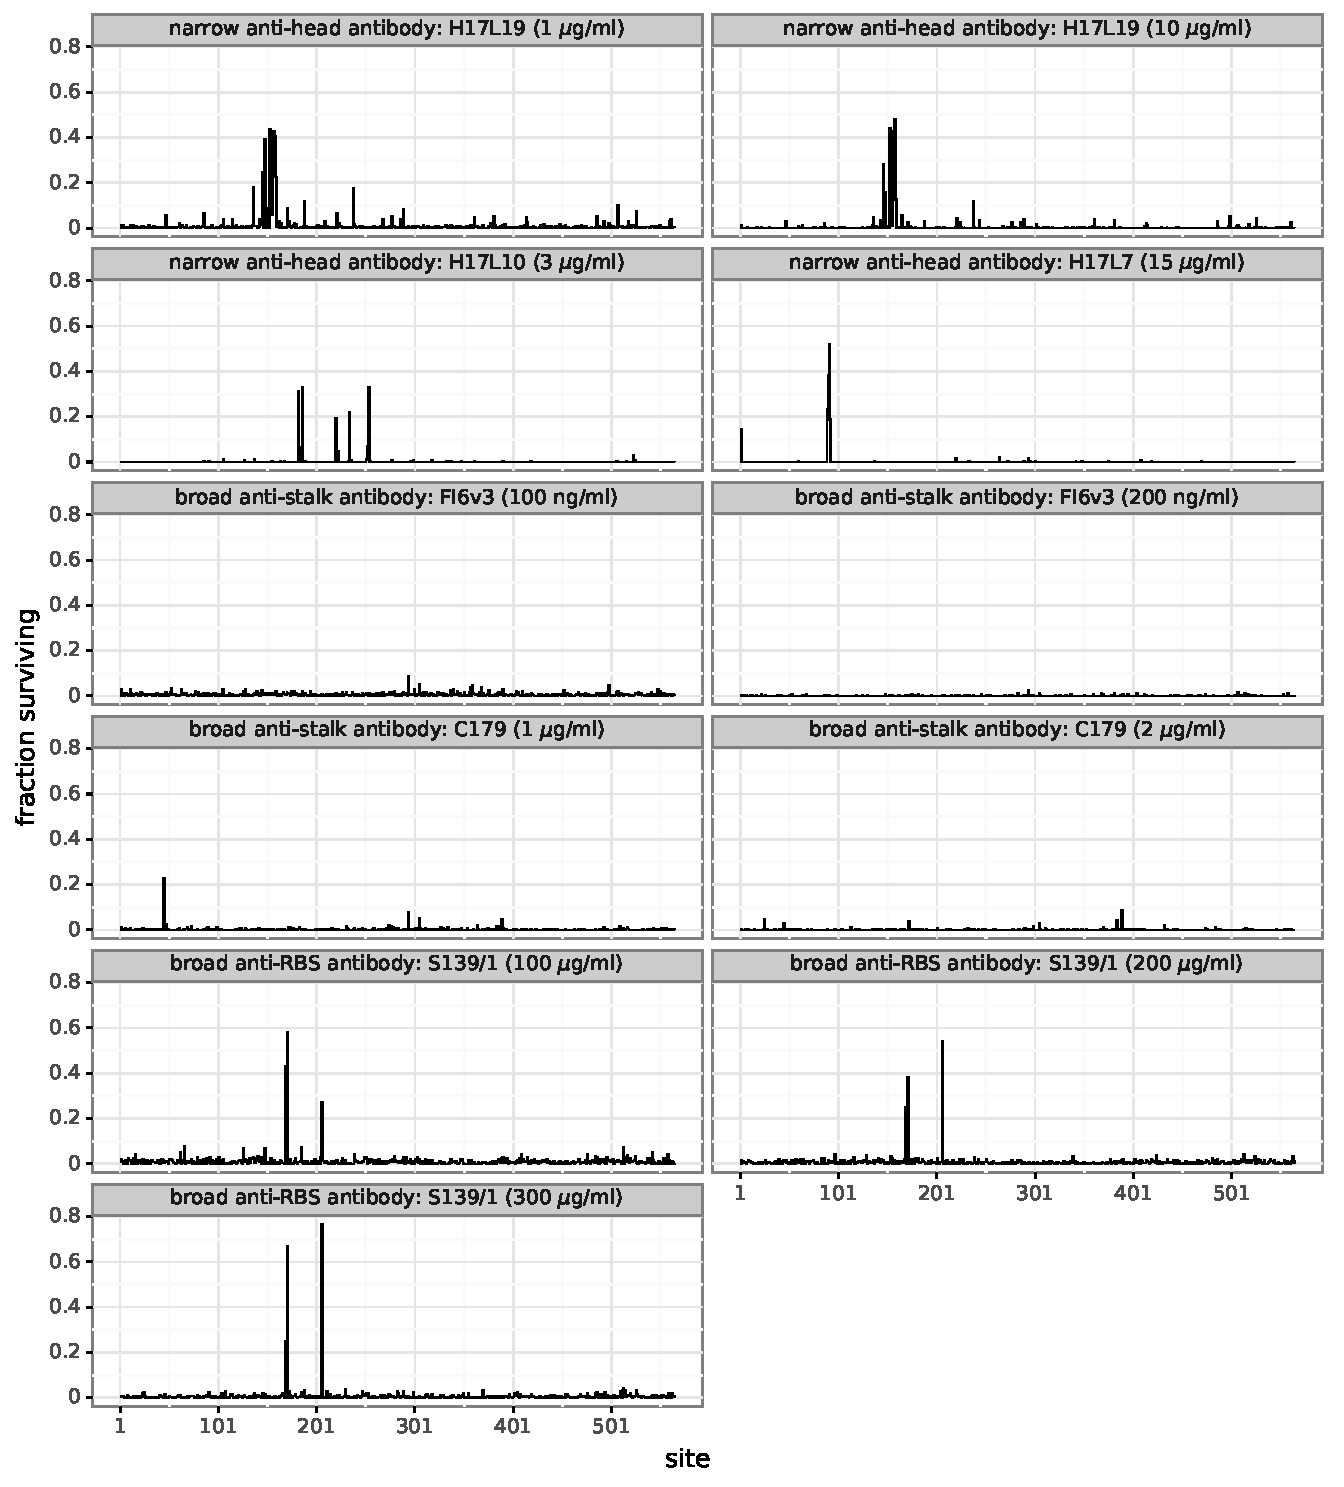
\includegraphics[width=\textwidth]{figs/maxfracsurvive.pdf}}
\caption{\label{suppfig:maxfracsurvive}
{\bf The excess fraction surviving for the single strongest escape mutation at each site.}
This plot differs from Figure~\ref{fig:avgfracsurvive} in that the height of the line indicates the excess fraction of virions that survive the antibody selection for the single strongest escape mutation at that site, rather than the average across all amino-acid mutations at that site.
}
\end{suppfigure}

\begin{suppfigure}
\centerline{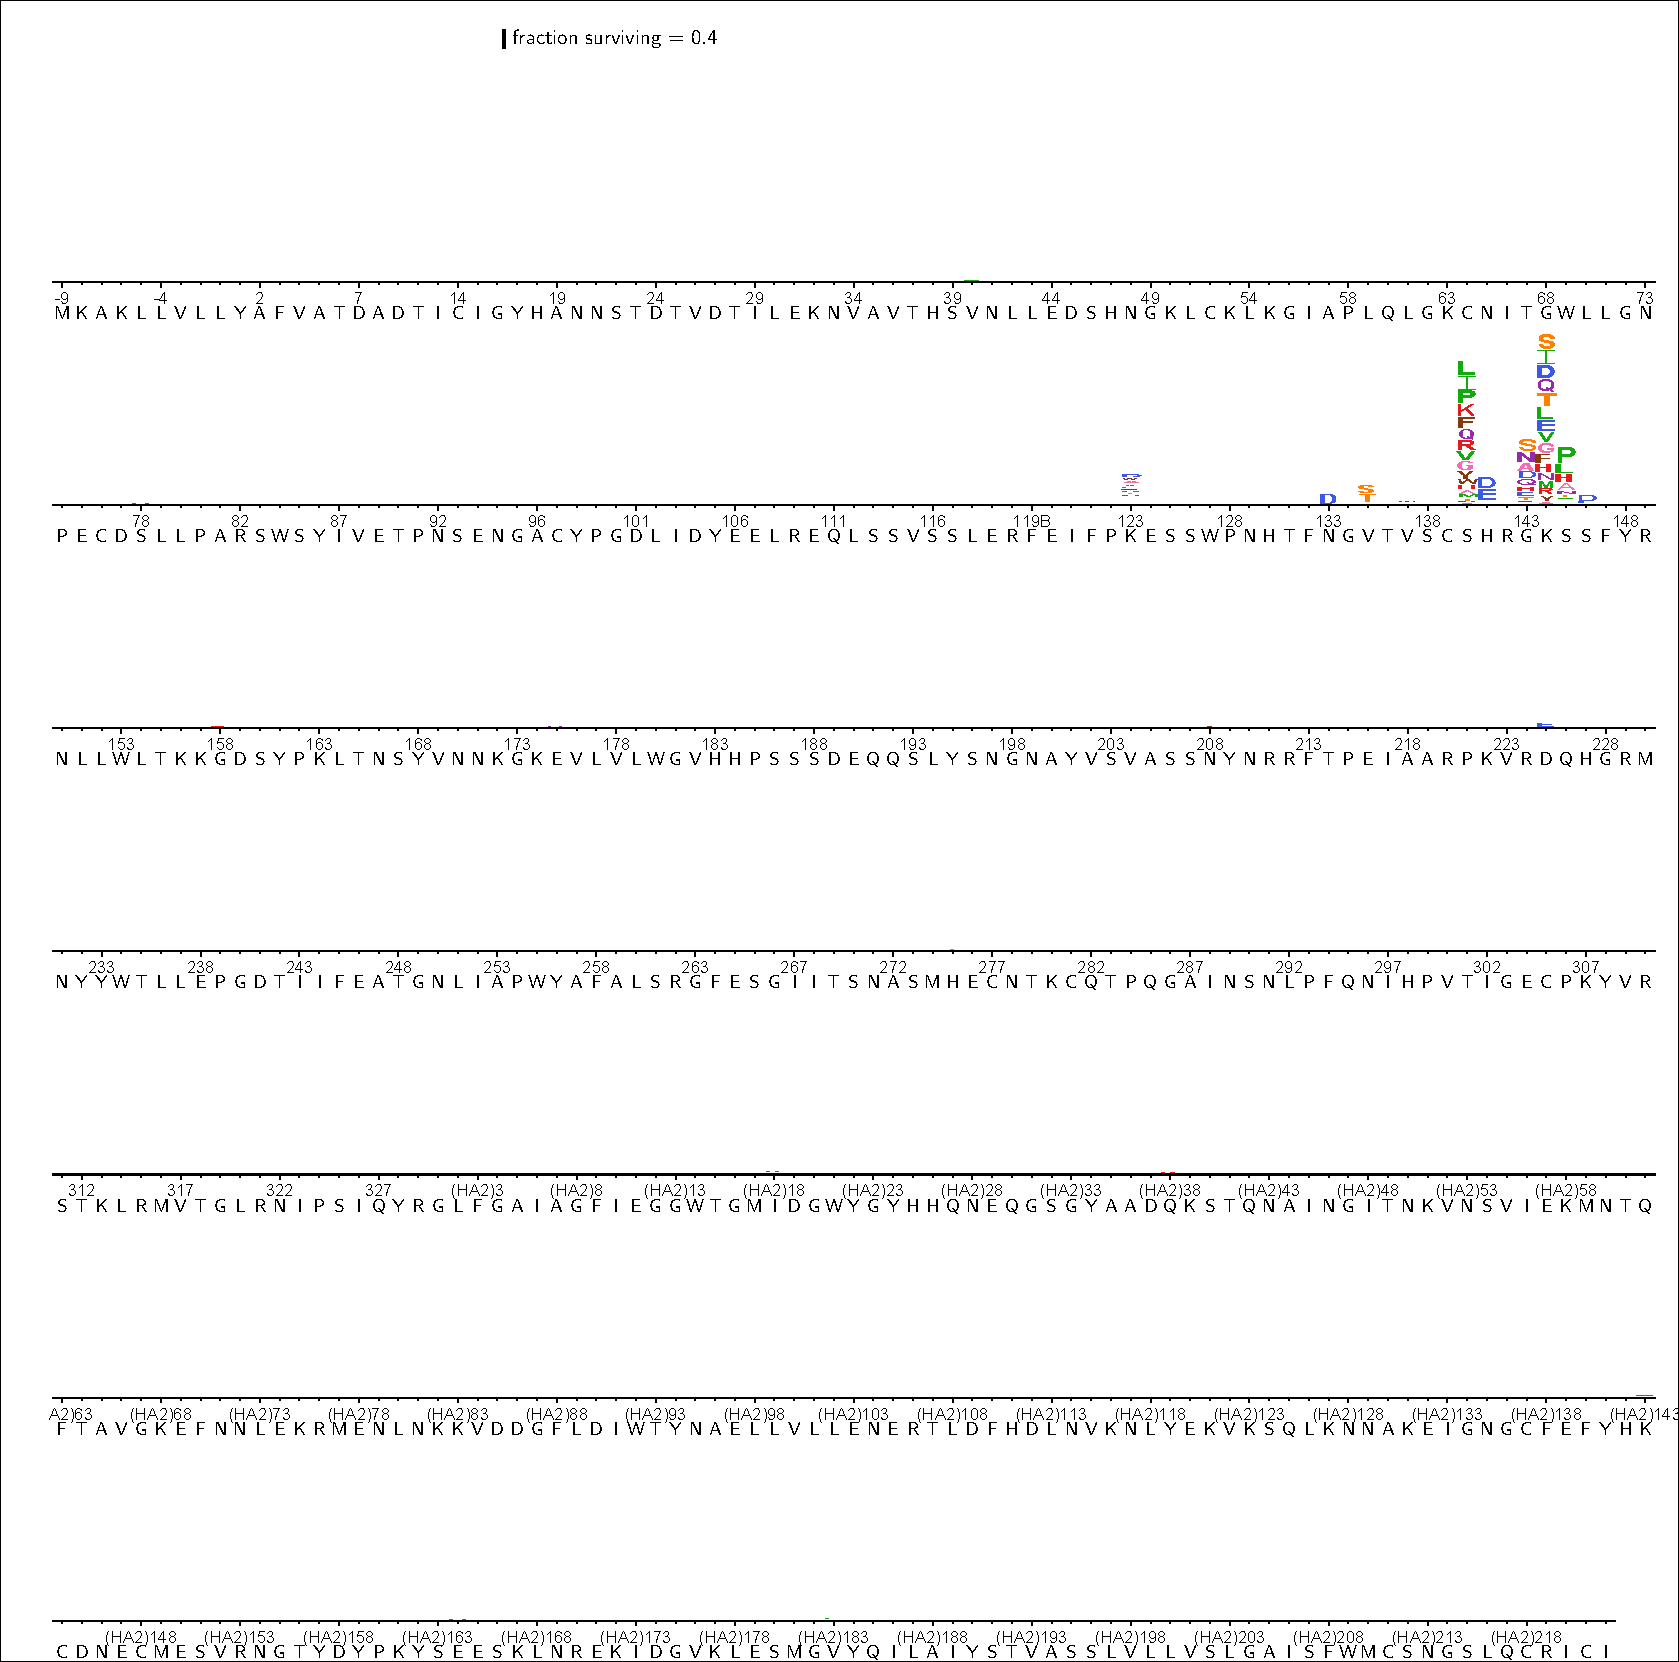
\includegraphics[trim=0.1cm 0.02cm 0.1cm 0.03cm,clip=true,width=\textwidth]{figs/logoplots/H17L19_fracsurvive.pdf}}
\caption{\label{suppfig:H17L19logo}
{\bf The excess fraction surviving selection with antibody H17L19 for all amino-acid mutations.}
The excess fraction surviving for each replicate was computed using Equation~\ref{eq:fracsurvive_excess}, then we took the median across all technical and biological replicates for each antibody concentration, and then took the medians of those values across concentrations.
The height of each letter is proportional to the excess fraction surviving of virions with that mutation.
The scale bar at the top of the plot relates the letter heights to the actual fractions.
The sites are labeled using H3 numbering.
}
\end{suppfigure}

\begin{suppfigure}
\centerline{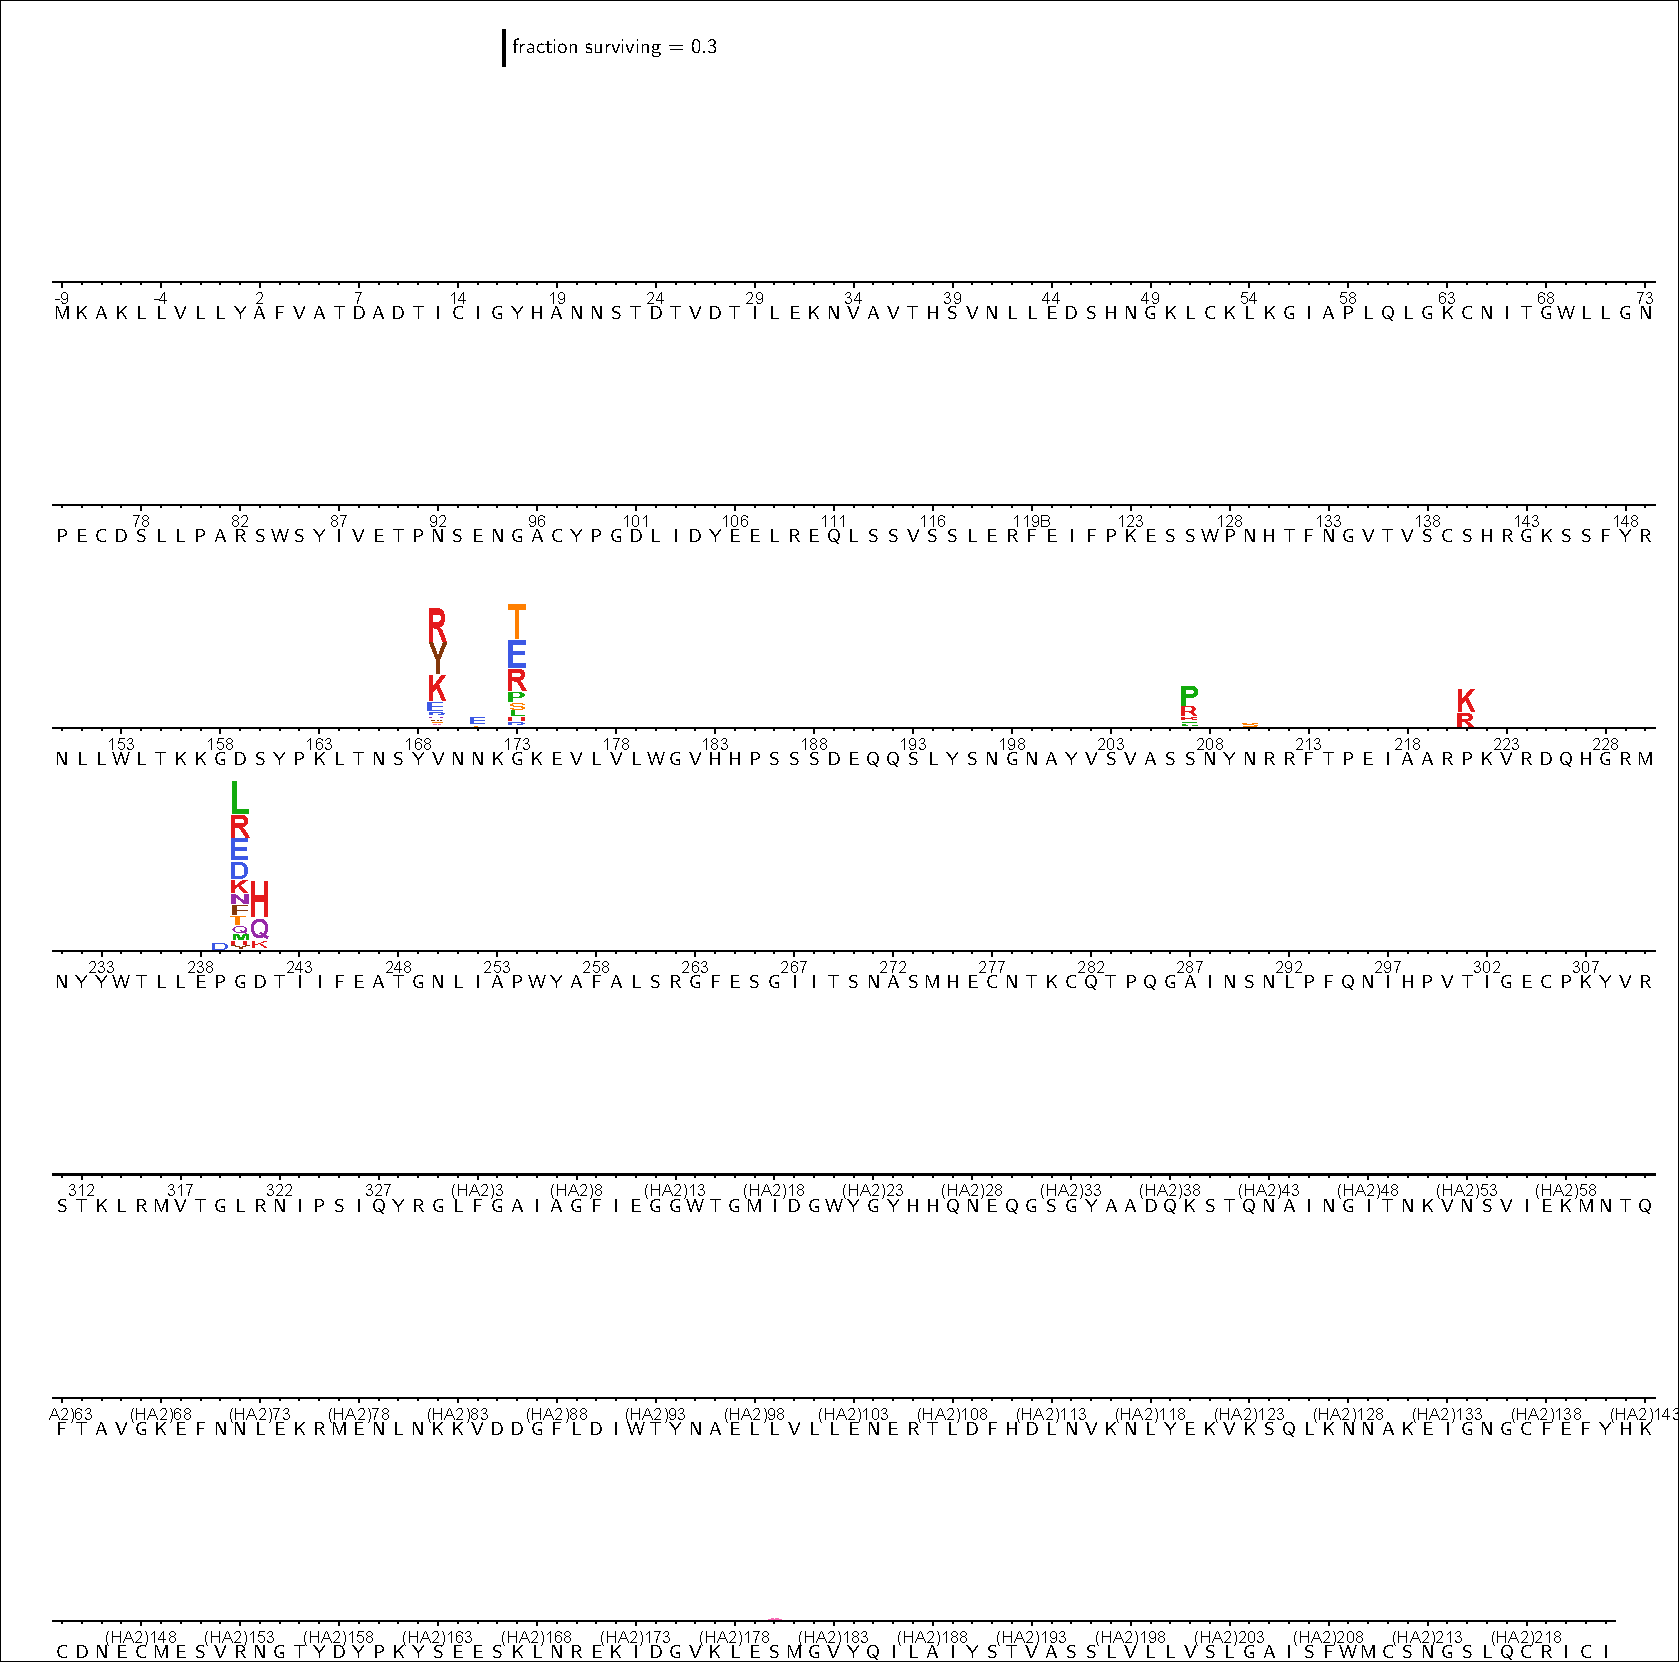
\includegraphics[trim=0.1cm 0.02cm 0.1cm 0.03cm,clip=true,width=\textwidth]{figs/logoplots/H17L10_fracsurvive.pdf}}
\caption{\label{suppfig:H17L10logo}
{\bf The excess fraction surviving selection with antibody H17L10 for all amino-acid mutations.}
The excess fraction surviving for each replicate was computed using Equation~\ref{eq:fracsurvive_excess}, then we took the median across all technical and biological replicates for each antibody concentration, and then took the medians of those values across concentrations.
The height of each letter is proportional to the excess fraction surviving of virions with that mutation.
The scale bar at the top of the plot relates the letter heights to the actual fractions.
The sites are labeled using H3 numbering.
}
\end{suppfigure}

\begin{suppfigure}
\centerline{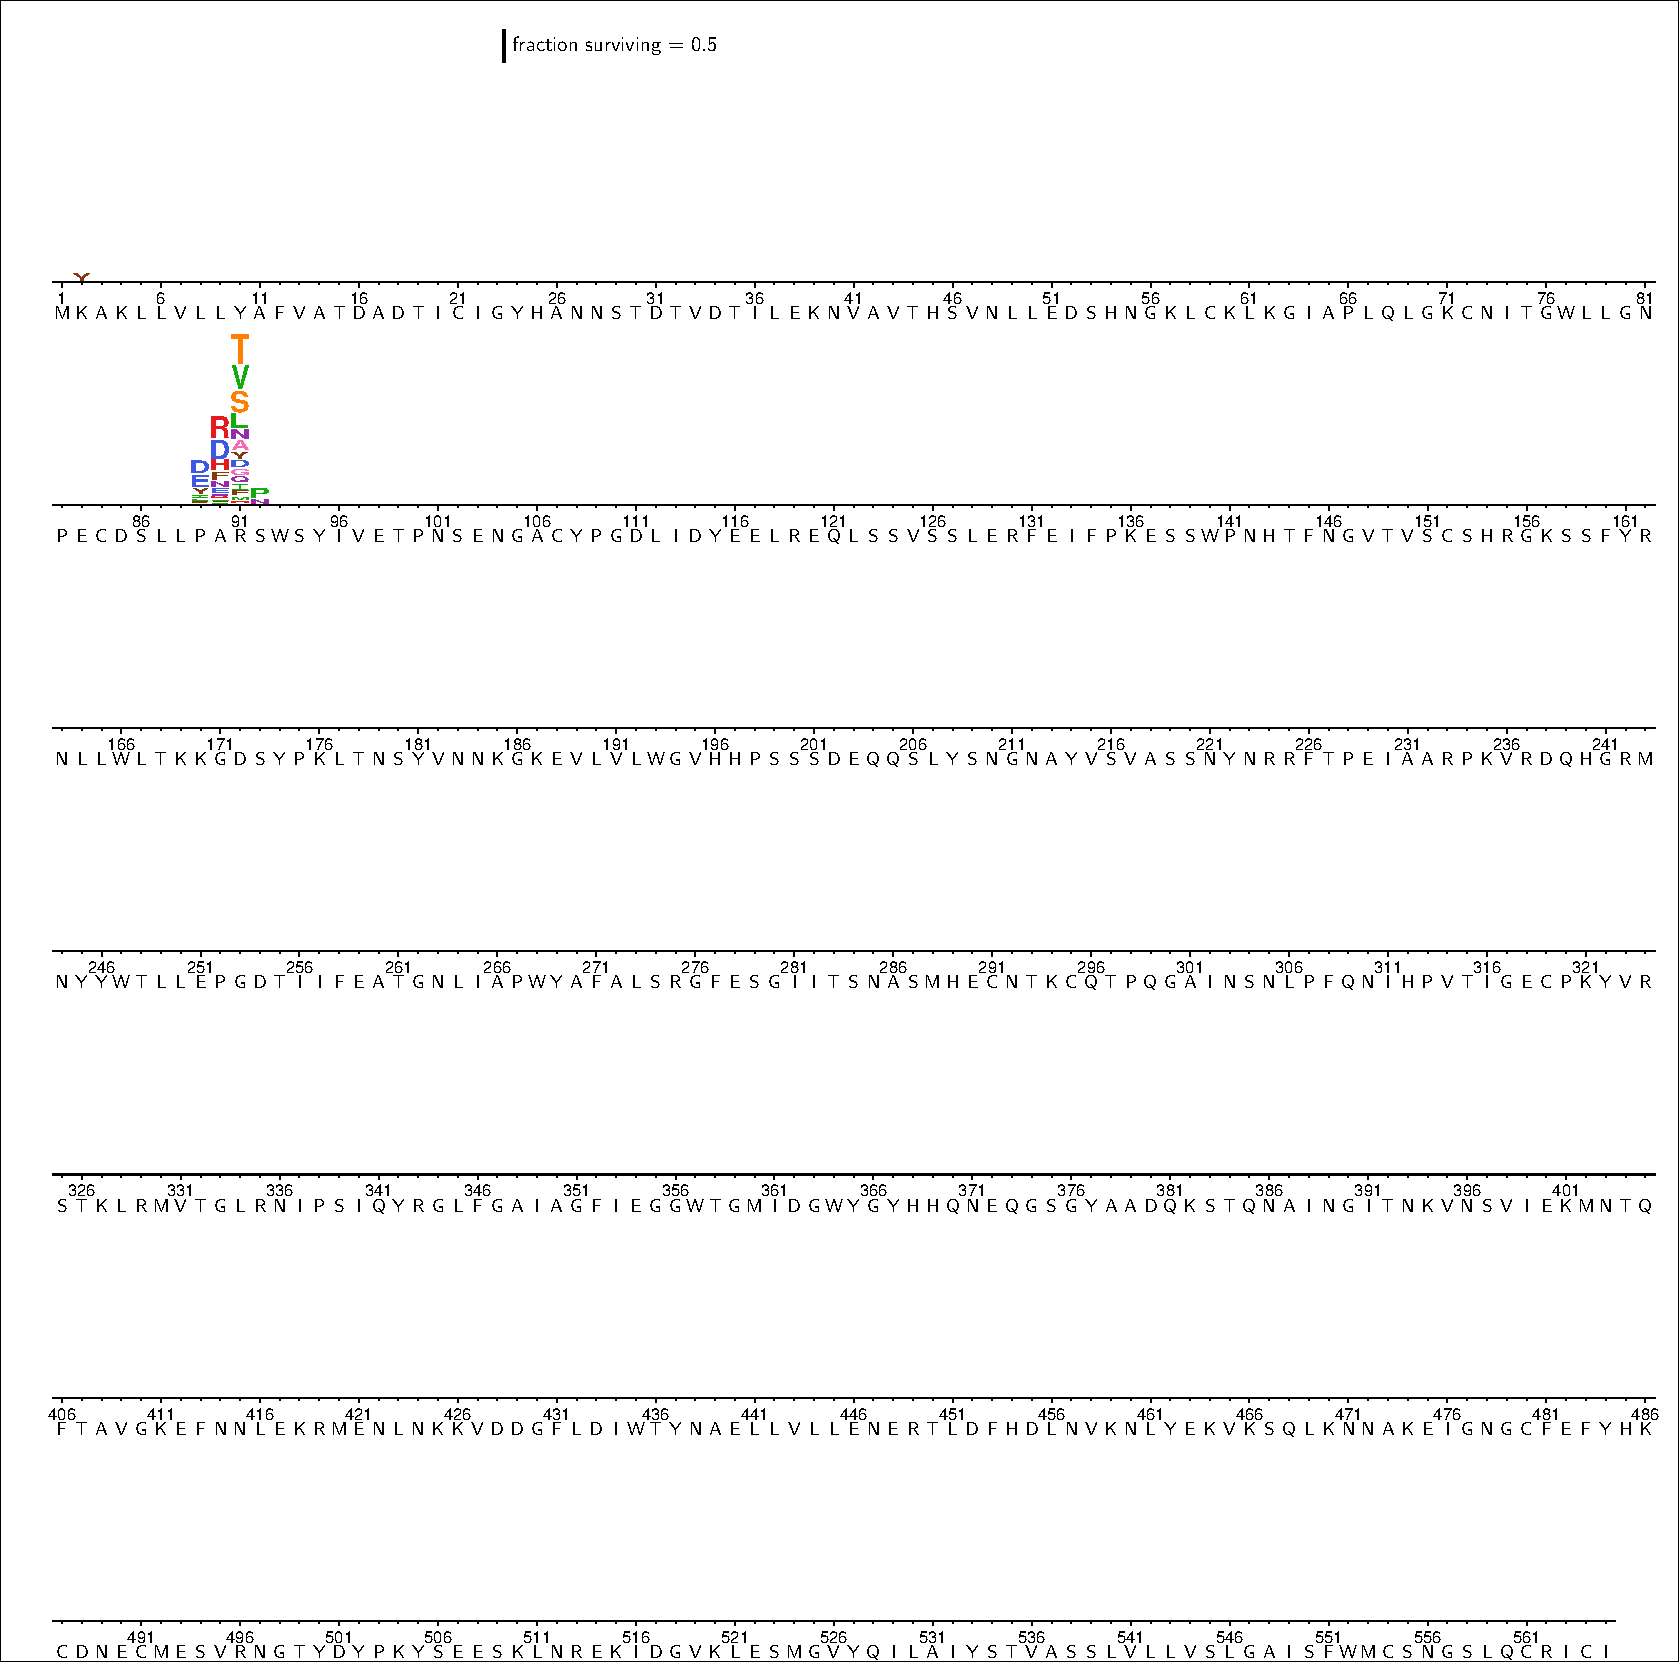
\includegraphics[trim=0.1cm 0.02cm 0.1cm 0.03cm,clip=true,width=\textwidth]{figs/logoplots/H17L7_fracsurvive.pdf}}
\caption{\label{suppfig:H17L7logo}
{\bf The excess fraction surviving selection with antibody H17L7 for all amino-acid mutations.}
The excess fraction surviving for each replicate was computed using Equation~\ref{eq:fracsurvive_excess}, then we took the median across all technical and biological replicates for each antibody concentration, and then took the medians of those values across concentrations.
The height of each letter is proportional to the excess fraction surviving of virions with that mutation.
The scale bar at the top of the plot relates the letter heights to the actual fractions.
The sites are labeled using H3 numbering.
}
\end{suppfigure}

\begin{suppfigure}
\centerline{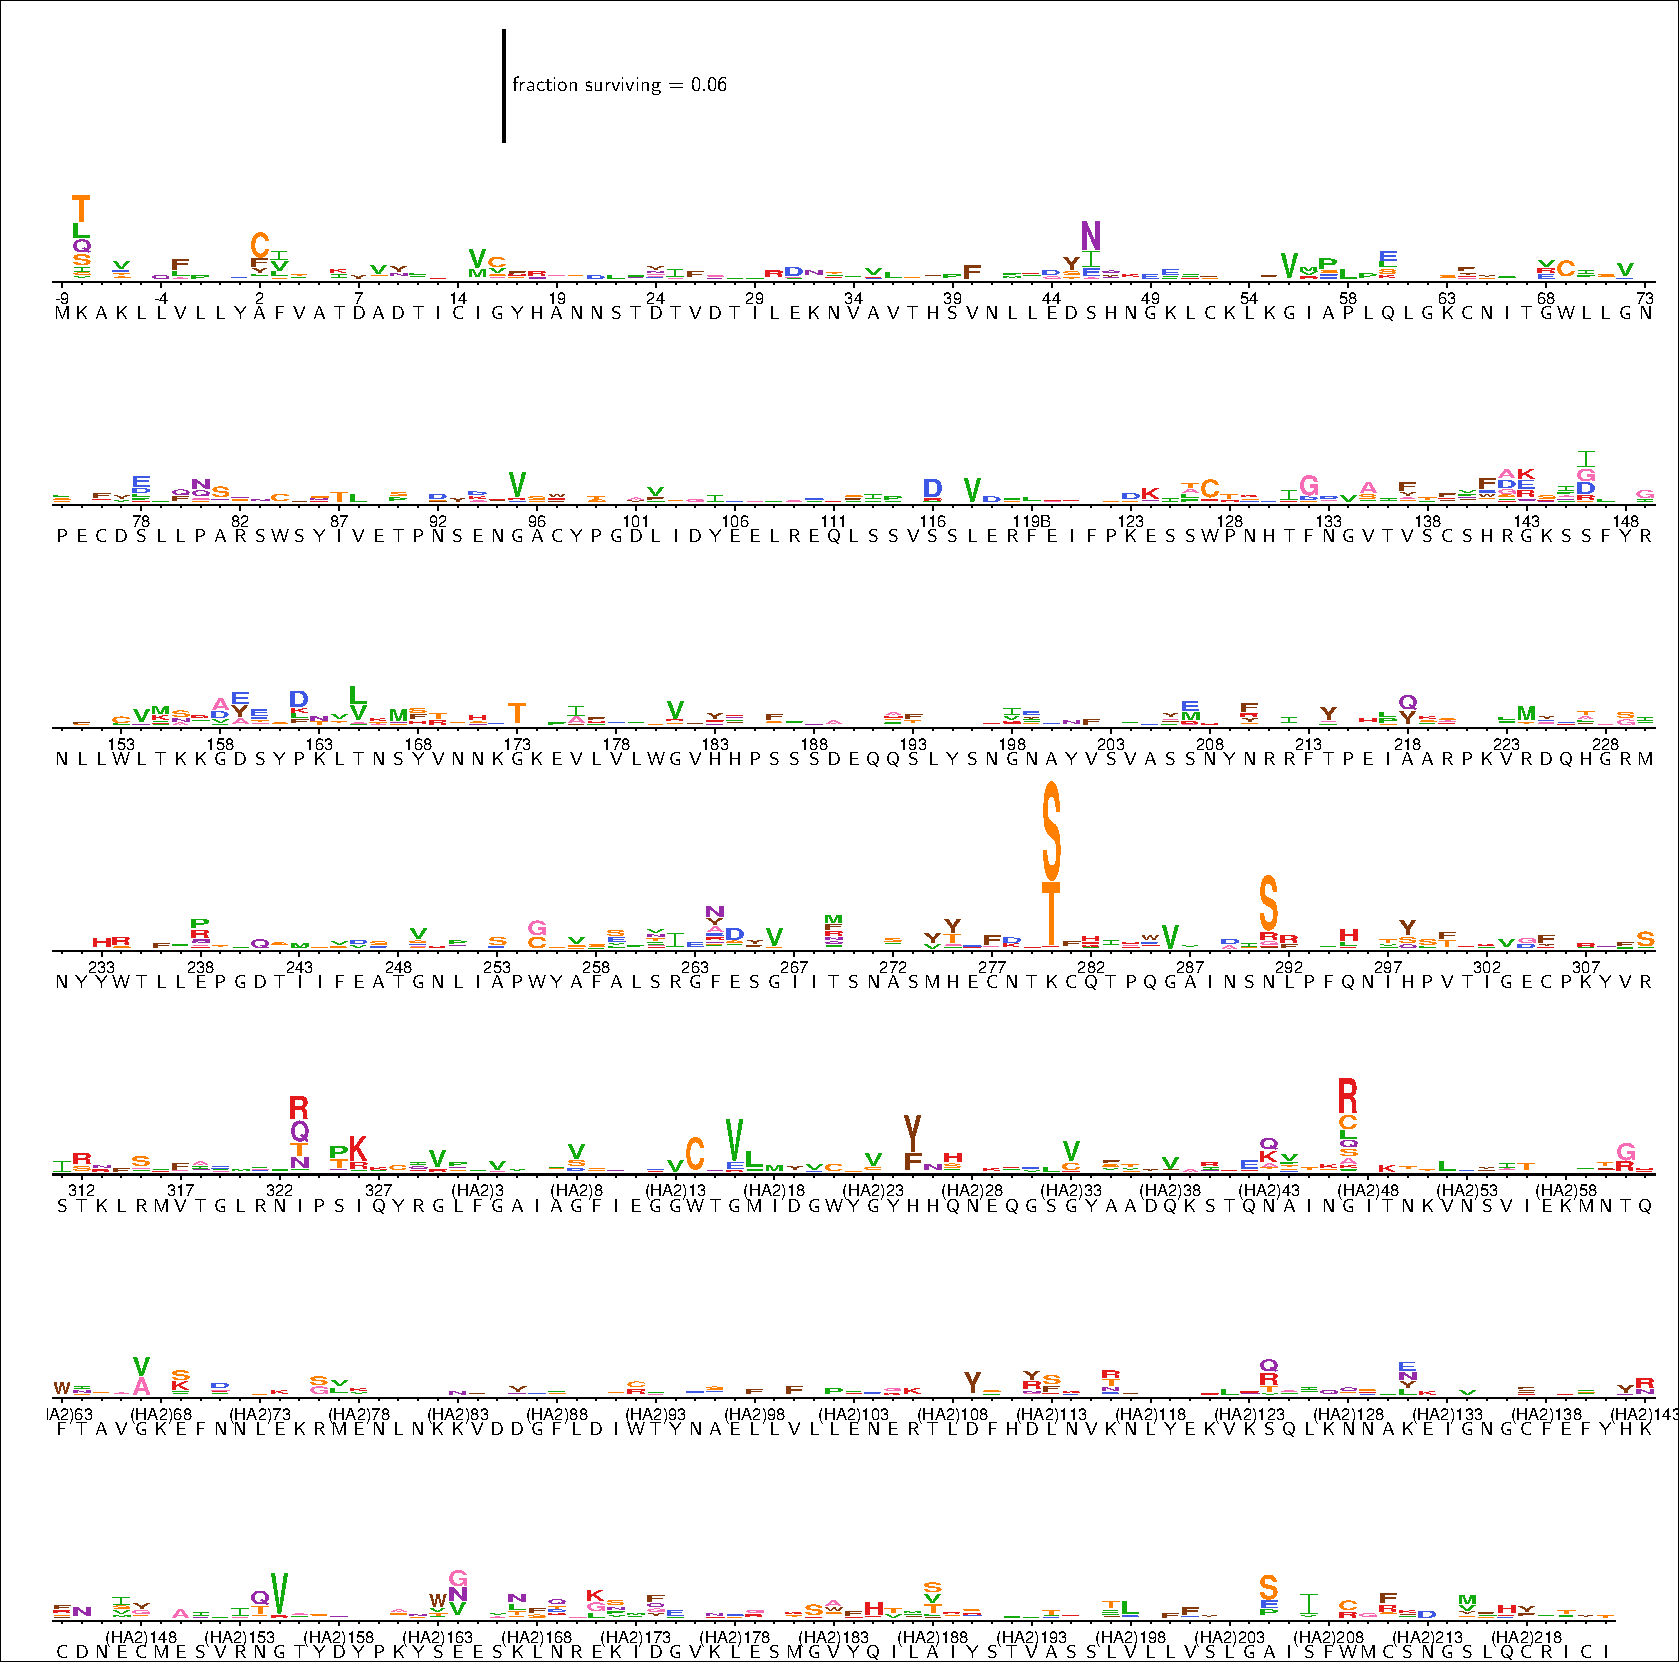
\includegraphics[trim=0.1cm 0.02cm 0.1cm 0.03cm,clip=true,width=\textwidth]{figs/logoplots/FI6v3_fracsurvive.pdf}}
\caption{\label{suppfig:FI6v3logo}
{\bf The excess fraction surviving selection with antibody FI6v3 for all amino-acid mutations.}
The excess fraction surviving for each replicate was computed using Equation~\ref{eq:fracsurvive_excess}, then we took the median across all technical and biological replicates for each antibody concentration, and then took the medians of those values across concentrations.
The height of each letter is proportional to the excess fraction surviving of virions with that mutation.
The scale bar at the top of the plot relates the letter heights to the actual fractions.
The sites are labeled using H3 numbering.
}
\end{suppfigure}

\begin{suppfigure}
\centerline{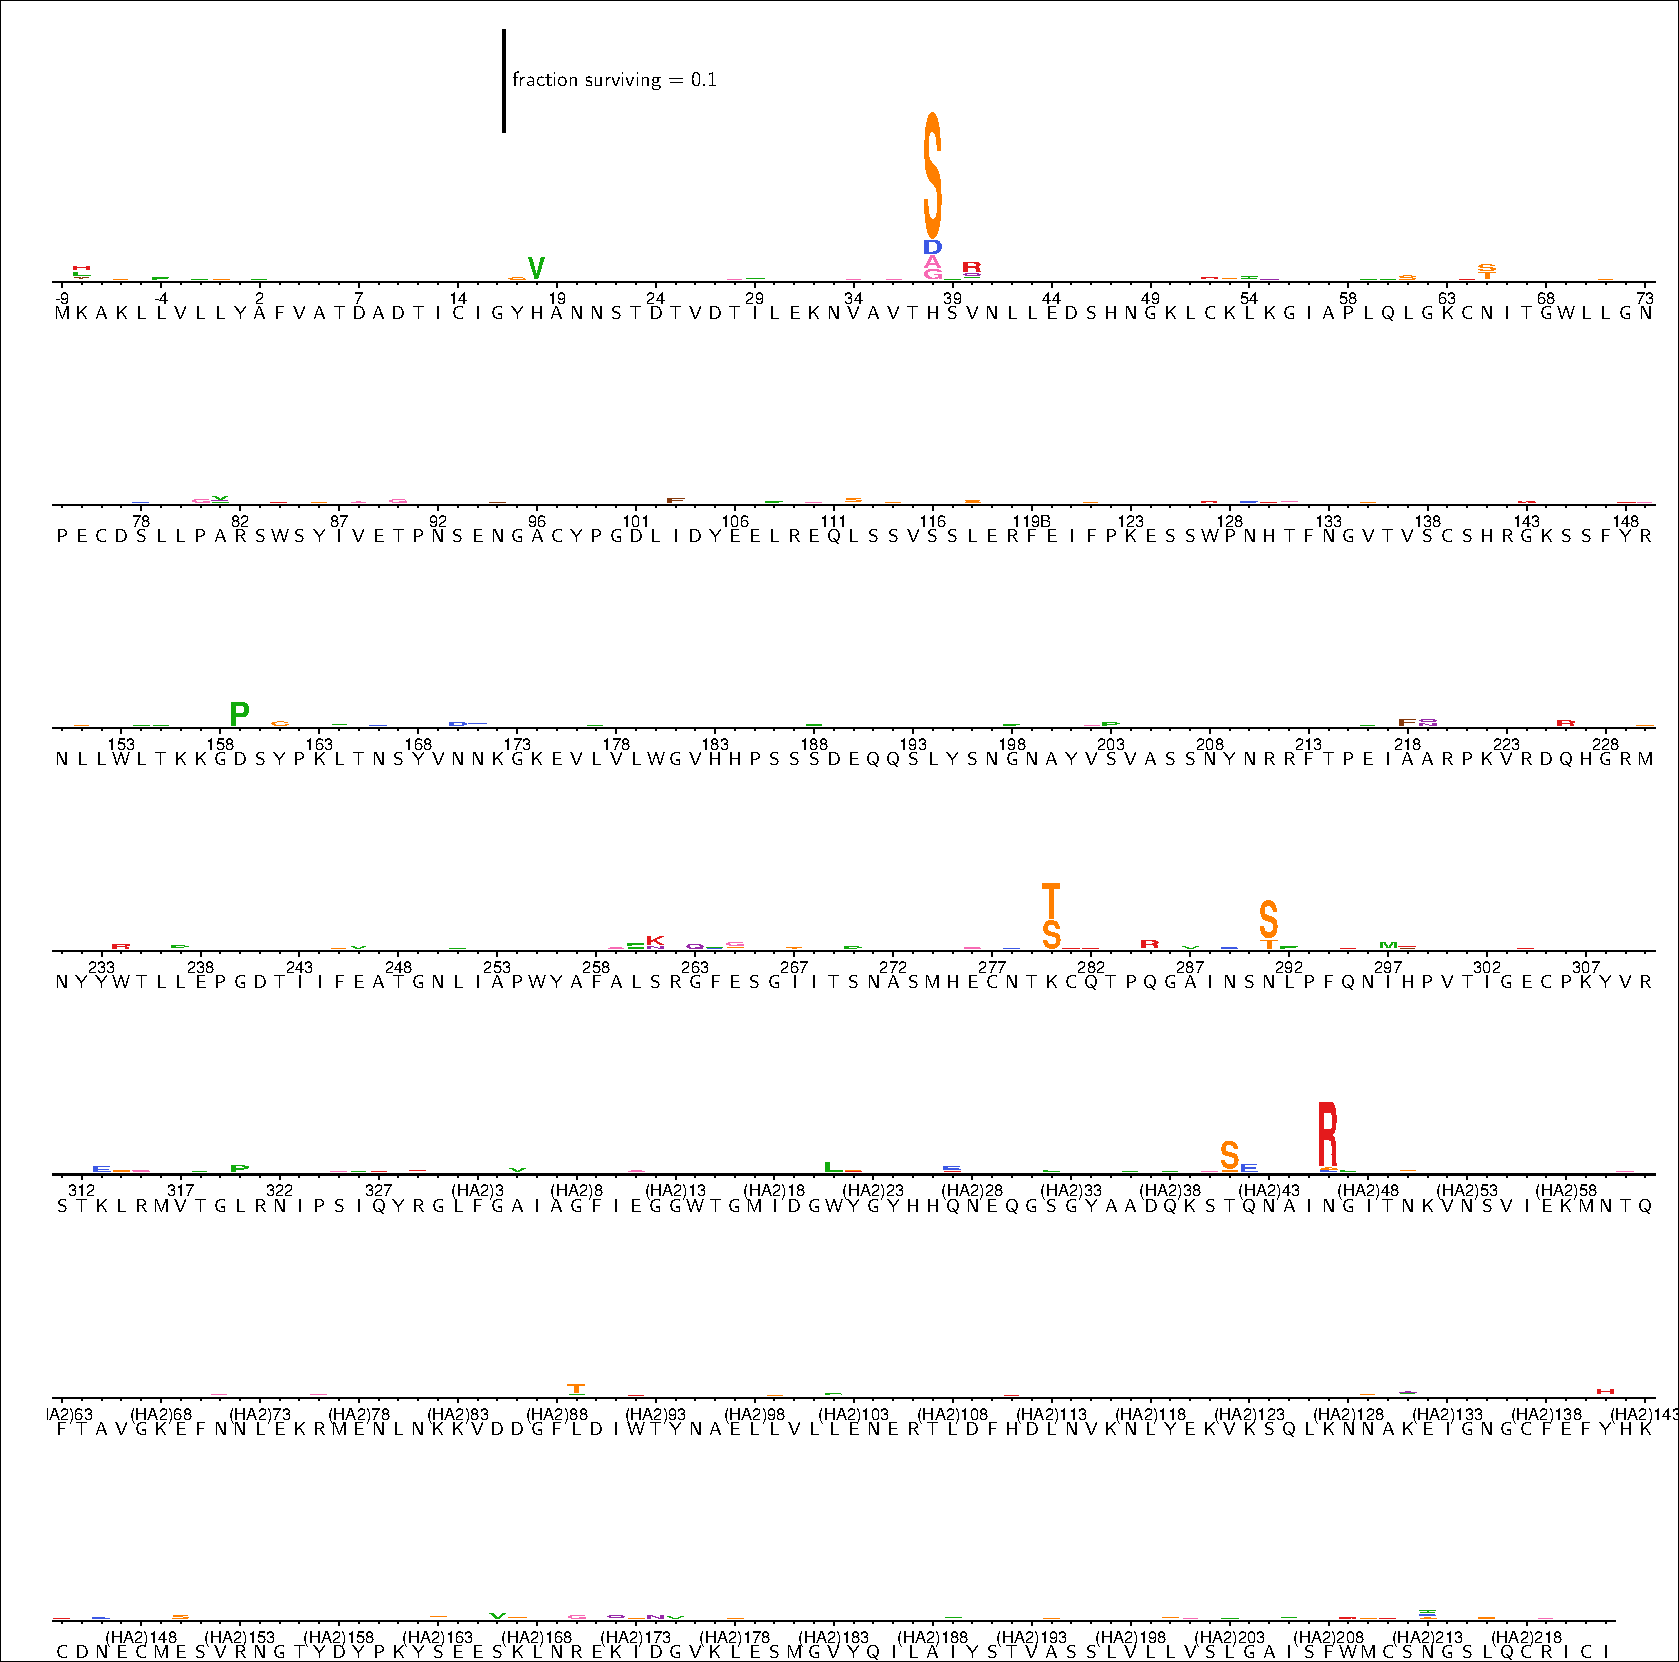
\includegraphics[trim=0.1cm 0.02cm 0.1cm 0.03cm,clip=true,width=\textwidth]{figs/logoplots/C179_fracsurvive.pdf}}
\caption{\label{suppfig:C179logo}
{\bf The excess fraction surviving selection with antibody C179 for all amino-acid mutations.}
The excess fraction surviving for each replicate was computed using Equation~\ref{eq:fracsurvive_excess}, then we took the median across all technical and biological replicates for each antibody concentration, and then took the medians of those values across concentrations.
The height of each letter is proportional to the excess fraction surviving of virions with that mutation.
The scale bar at the top of the plot relates the letter heights to the actual fractions.
The sites are labeled using H3 numbering.
}
\end{suppfigure}

\begin{suppfigure}
\centerline{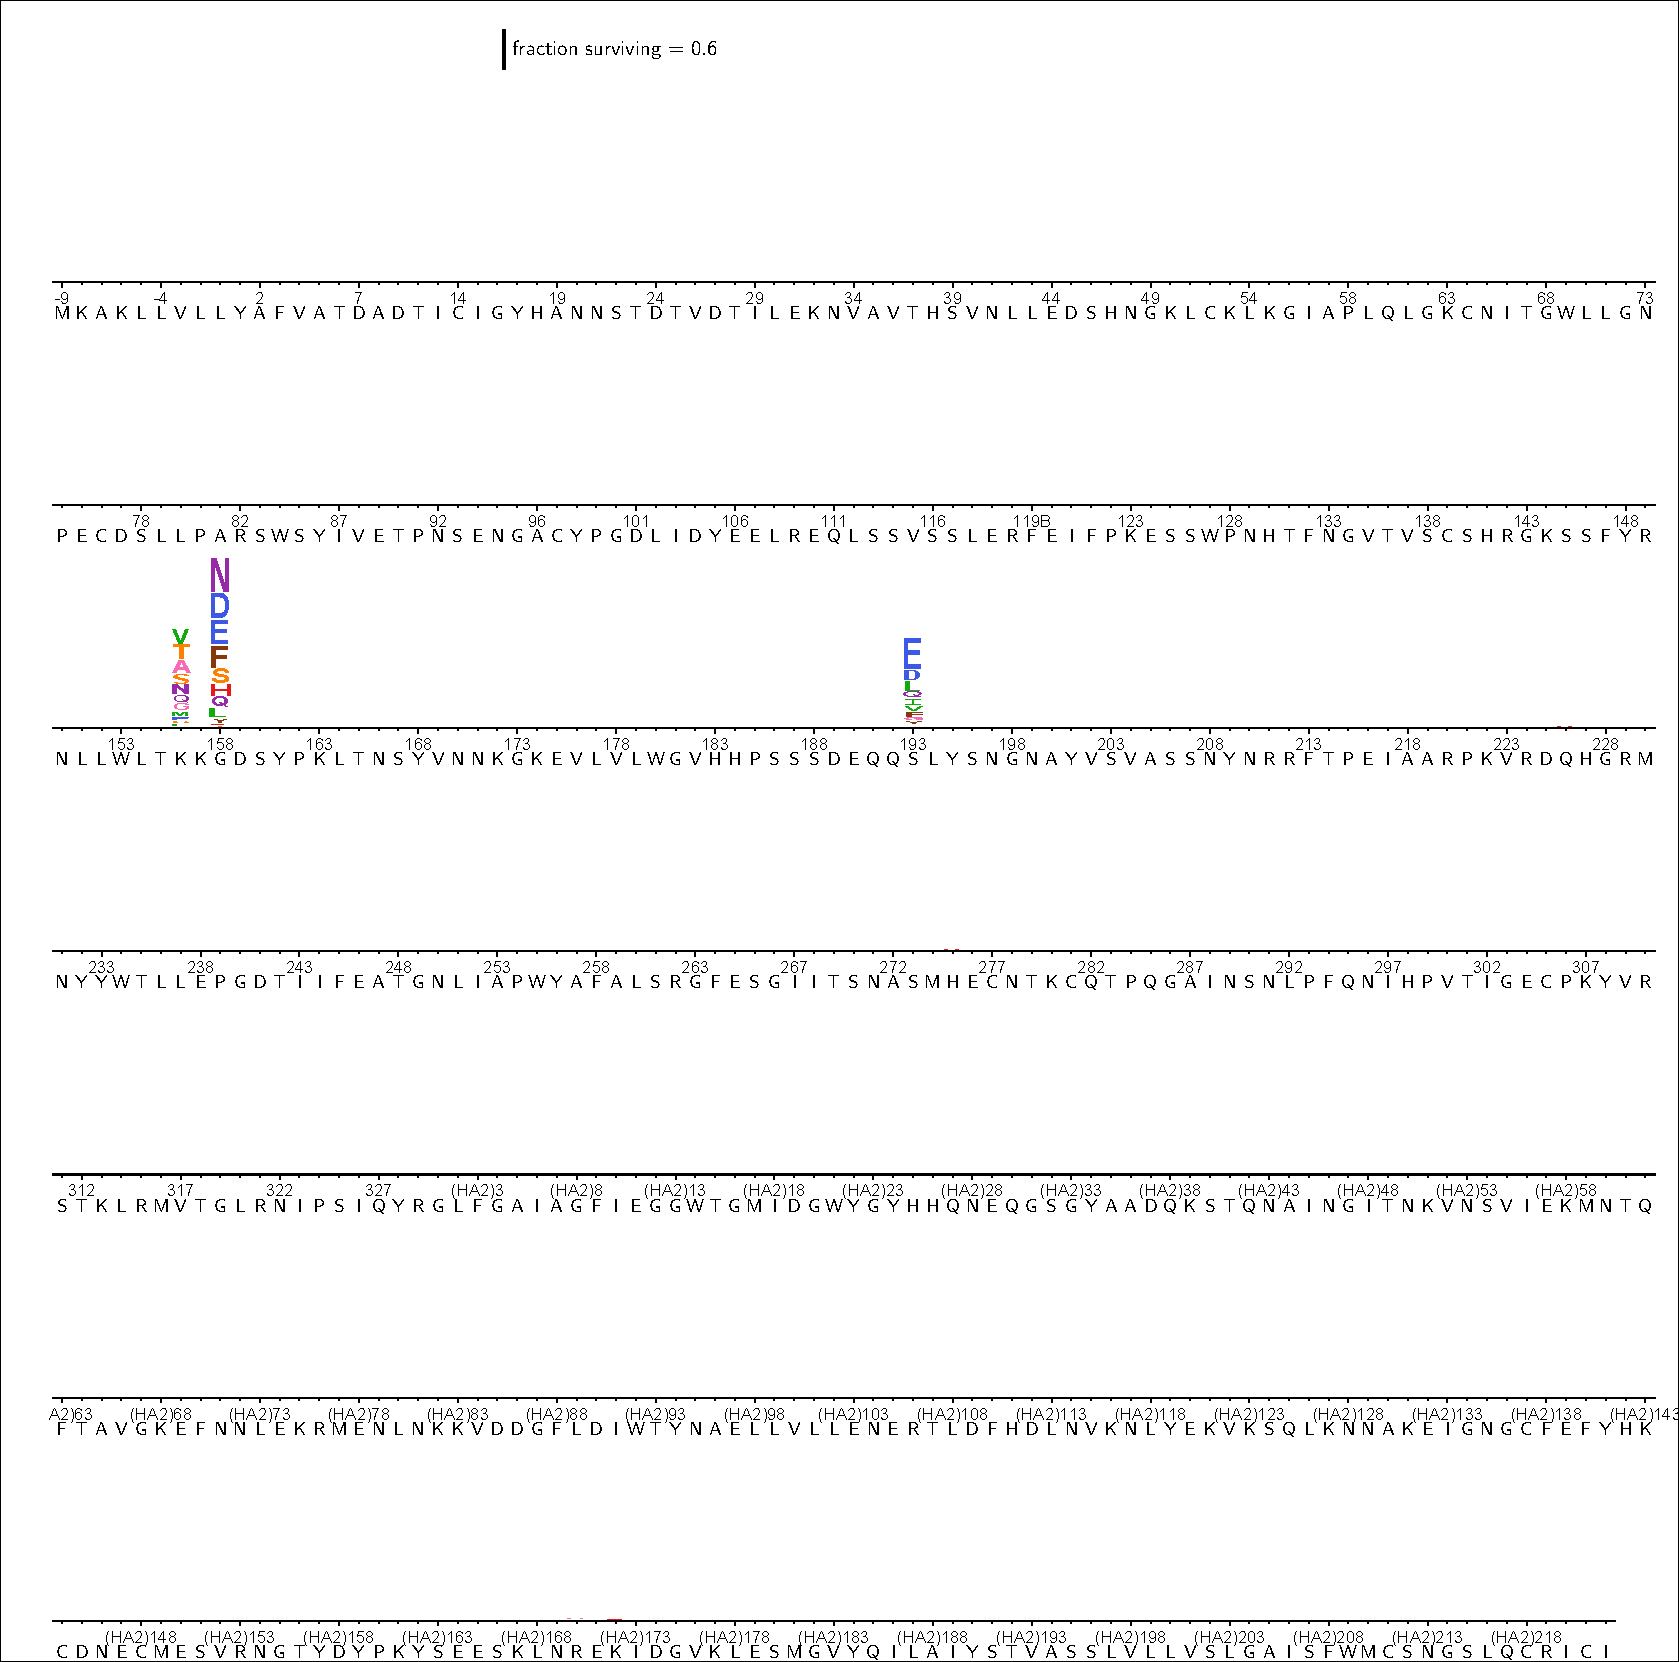
\includegraphics[trim=0.1cm 0.02cm 0.1cm 0.03cm,clip=true,width=\textwidth]{figs/logoplots/S139_fracsurvive.pdf}}
\caption{\label{suppfig:S139logo}
{\bf The excess fraction surviving selection with antibody S139/1 for all amino-acid mutations.}
The excess fraction surviving for each replicate was computed using Equation~\ref{eq:fracsurvive_excess}, then we took the median across all technical and biological replicates for each antibody concentration, and then took the medians of those values across concentrations.
The height of each letter is proportional to the excess fraction surviving of virions with that mutation.
The scale bar at the top of the plot relates the letter heights to the actual fractions.
The sites are labeled using H3 numbering.
}
\end{suppfigure}

\end{document}
